% =====================================================================================
% RegimeStress --- Paper 2 of the Trivijaya Quant Research programme.
%
% Every number in this paper resolves through a generated macro. Nothing is transcribed.
%
%   papers/regimestress_numbers.tex <- scripts/build_paper_numbers.py        (\rs...)
%   papers/programme_numbers.tex    <- scripts/build_programme_numbers.py    (\pgm...)
%   papers/figures/*.png            <- scripts/build_paper_figures.py
%
% Compile: pdflatex regimestress && pdflatex regimestress   (twice, for the contents)
% =====================================================================================
\documentclass[11pt,a4paper]{article}

\newcommand{\paperName}{RegimeStress}
\newcommand{\paperSubtitle}{A strategy survived one history.\\ When does it break?}
\newcommand{\paperNumber}{2}
\newcommand{\paperShortHead}{Validity $\rightarrow$ robustness}

% =====================================================================================
% Shared style for the three papers of the Trivijaya Quant Research programme.
%
% The three papers report one programme and must look like it: same typography, same
% heading hierarchy, same table rules, same panel vocabulary, same cover structure.
% Anything paper-specific (title, running head, abstract) stays in the paper's own file.
%
% Each paper defines, BEFORE inputting this file:
%   \paperName        e.g. AlphaAudit
%   \paperSubtitle    the one-line question the paper answers
%   \paperNumber      1, 2 or 3
%   \paperShortHead   the right-hand running head
% =====================================================================================

\usepackage[utf8]{inputenc}
\usepackage[T1]{fontenc}
\usepackage{lmodern}
\usepackage[scaled=0.92]{helvet}          % sans face, headings only
\usepackage[margin=1.05in,top=1.15in,bottom=1.1in]{geometry}
\usepackage{microtype}
\usepackage{amsmath,amssymb}
\usepackage{booktabs}
\usepackage{array}
\usepackage{graphicx}
\usepackage{xcolor}
\usepackage[most]{tcolorbox}
\usepackage{titlesec}
\usepackage{enumitem}
\usepackage[font=small,labelfont={bf,color=navy},labelsep=period]{caption}
\usepackage{fancyhdr}
\usepackage{natbib}
\usepackage[colorlinks=true]{hyperref}   % loaded last, as hyperref requires

% The rupee sign is not in the default T1 encoding. A plain "Rs." is unambiguous, renders
% identically on every machine, and avoids a font dependency a reader would have to satisfy
% before they could compile the paper that asks them to check our numbers.
\providecommand{\rupee}{\textrm{Rs.}\,}

% ---- Palette: white ground, blues, one warm accent for our own errors ---------------
\definecolor{navy}{HTML}{0E2E5C}
\definecolor{steel}{HTML}{2C6BA8}
\definecolor{sky}{HTML}{5B93C7}
\definecolor{mist}{HTML}{F0F5FB}
\definecolor{ash}{HTML}{F6F7F9}
\definecolor{ink}{HTML}{1A1A1A}
\definecolor{rust}{HTML}{9C4221}

\color{ink}
\hypersetup{linkcolor=steel, citecolor=steel, urlcolor=steel}

% ---- Repository, cited often enough to deserve one definition ----------------------
\newcommand{\repourl}{https://github.com/Ashwin-aadi/Trivijaya-Quant-Research}
\newcommand{\repo}{\href{\repourl}{\texttt{github.com/Ashwin-aadi/Trivijaya-Quant-Research}}}
\newcommand{\siteurl}{https://ashwin-aadi.github.io/Trivijaya-Quant-Research/}
\newcommand{\site}{\href{\siteurl}{\texttt{ashwin-aadi.github.io/Trivijaya-Quant-Research}}}

% ---- Headings ----------------------------------------------------------------------
\newcommand{\sectionrule}{{\color{sky}\rule{\linewidth}{0.5pt}}\vspace{-0.9em}}
\titleformat{\section}[block]
  {\sffamily\large\bfseries\color{navy}}
  {\colorbox{navy}{\textcolor{white}{\sffamily\bfseries\ \thesection\ }}}{0.7em}{}
  [\vspace{0.25em}\sectionrule]
\titleformat{\subsection}[block]
  {\sffamily\normalsize\bfseries\color{navy}}{\thesubsection}{0.6em}{}
\titleformat{\paragraph}[runin]
  {\sffamily\bfseries\color{navy}}{}{0em}{}[\;]
\titlespacing*{\section}{0pt}{1.6em}{0.8em}
\titlespacing*{\subsection}{0pt}{1.2em}{0.5em}

% ---- Running head ------------------------------------------------------------------
\pagestyle{fancy}\fancyhf{}
\renewcommand{\headrulewidth}{0.4pt}
\renewcommand{\headrule}{{\color{sky}\hrule height 0.4pt}}
\fancyhead[L]{\sffamily\scriptsize\color{navy}\MakeUppercase{\paperName}}
\fancyhead[R]{\sffamily\scriptsize\color{navy}\paperShortHead}
\fancyfoot[C]{\sffamily\scriptsize\color{navy}\thepage}
\fancypagestyle{plain}{\fancyhf{}\renewcommand{\headrulewidth}{0pt}
  \fancyfoot[C]{\sffamily\scriptsize\color{navy}\thepage}}

% ---- Panels ------------------------------------------------------------------------
% A finding the reader must not skim past.
\newtcolorbox{finding}[1][]{
  enhanced, breakable, colback=mist, colframe=steel, boxrule=0pt,
  leftrule=2.5pt, arc=1pt, left=9pt, right=9pt, top=7pt, bottom=7pt,
  coltext=navy, fonttitle=\sffamily\bfseries\small, #1}

% A place where we report our own error. Deliberately a different colour from the findings,
% so a reader flipping through can see at a glance that the paper contains both.
\newtcolorbox{selfreport}[1][]{
  enhanced, breakable, colback=ash, colframe=rust, boxrule=0pt,
  leftrule=2.5pt, arc=1pt, left=9pt, right=9pt, top=7pt, bottom=7pt,
  fonttitle=\sffamily\bfseries\small, #1}

% What a result does *not* license. Every headline in this programme has one of these, because
% the distance between "we measured X on our corpus" and "X is true of AI" is where this
% literature goes wrong.
\newtcolorbox{scopebox}[1][]{
  enhanced, breakable, colback=white, colframe=sky, boxrule=0.6pt,
  arc=1pt, left=9pt, right=9pt, top=6pt, bottom=6pt,
  fonttitle=\sffamily\bfseries\small, title={\sffamily\bfseries What this does not say}, #1}

\newcommand{\keyfinding}[1]{\begin{finding}#1\end{finding}}

% A one-line takeaway that sits directly against a figure or table.
\newcommand{\takeaway}[1]{%
  \vspace{-0.4em}\noindent{\small\sffamily\color{navy}\textbf{Takeaway.}\ #1}\vspace{0.5em}}

% ---- Tables ------------------------------------------------------------------------
\newcommand{\thead}[1]{{\sffamily\bfseries\color{navy}#1}}
\renewcommand{\arraystretch}{1.15}

\setlist[itemize]{leftmargin=1.3em, itemsep=0.25em, topsep=0.4em}
\setlist[enumerate]{leftmargin=1.6em, itemsep=0.35em, topsep=0.4em}

% ---- Evidence-scope tags -----------------------------------------------------------
% The programme's central discipline: every finding is tagged with the population it was
% measured on, so a local-corpus observation can never be read as a statement about AI.
\newcommand{\tagbox}[2]{{\sffamily\scriptsize\textbf{\textcolor{#1}{[#2]}}}}
\newcommand{\taglocal}{\tagbox{steel}{LOCAL 7B}}
\newcommand{\tagfrontier}{\tagbox{navy}{FRONTIER}}
\newcommand{\tagmethod}{\tagbox{navy}{GENERATION METHOD}}
\newcommand{\tagindep}{\tagbox{rust}{GENERATOR-INDEPENDENT}}
\newcommand{\tagexpl}{\tagbox{rust}{EXPLORATORY}}
\newcommand{\tagprereg}{\tagbox{steel}{PRE-REGISTERED}}

% ---- Cover page --------------------------------------------------------------------
\newcommand{\programmecover}[1]{%
\begin{titlepage}
\thispagestyle{empty}
\raggedright
\vspace*{0.6in}
{\sffamily\small\color{steel}\MakeUppercase{Trivijaya Quant Research Programme}\\[0.2em]
 \color{sky}\rule{\linewidth}{1.2pt}}\\[0.3em]
{\sffamily\small\color{steel}Paper \paperNumber\ of 3 \quad$\cdot$\quad
 Measurement infrastructure for AI-driven quantitative research on Indian equities}

\vspace{1.5in}
{\sffamily\bfseries\color{navy}\fontsize{46}{50}\selectfont \paperName}\\[0.7em]
{\color{sky}\rule{0.4\linewidth}{2pt}}\\[0.9em]
{\sffamily\Large\color{navy} \paperSubtitle}

\vspace{0.9in}
{\sffamily\large\color{ink} Ashwin Jain}\\[0.35em]
{\rmfamily\small Department of Computer Science and Engineering\\
Motilal Nehru National Institute of Technology Allahabad\\
Prayagraj, India\\[0.2em]
\texttt{ashwinaadi2007@gmail.com}}

\vfill
{\small\sffamily\color{navy}#1}

\vspace{0.5em}
{\small\rmfamily Code, corpus, fixtures and evaluation protocol: \repo\\
Programme overview and results: \site}\\[0.6em]
{\sffamily\small\color{steel} 8 August 2026}
\end{titlepage}}

% ---- The trilogy map, printed identically in all three papers ----------------------
\newcommand{\trilogymap}{%
\begin{tcolorbox}[enhanced, colback=ash, colframe=sky, boxrule=0.6pt, arc=1pt,
  left=10pt, right=10pt, top=8pt, bottom=8pt]
\small\sffamily\color{navy}
\textbf{One programme, three questions.} Each paper answers the question the previous one
raises, on one shared universe, one shared cost model and one shared backtest engine.
\vspace{0.5em}

\begin{tabular}{@{}p{0.055\linewidth}p{0.22\linewidth}p{0.65\linewidth}@{}}
\textbf{1} & \textbf{AlphaAudit} & Can an AI produce a trading strategy that is real,
  rather than a plausible artefact of luck and leakage? \\[0.3em]
\textbf{2} & \textbf{RegimeStress} & If a strategy looks real, when does it break? \\[0.3em]
\textbf{3} & \textbf{FlowState} & If a strategy survives, how much capital can it absorb? \\
\end{tabular}
\vspace{0.4em}

\textbf{Code $\rightarrow$ validity $\rightarrow$ robustness $\rightarrow$ scale.} The
programme's overarching question is whether making the AI better makes the \emph{research}
better --- and the three papers answer it only to the extent their experiments support.
\end{tcolorbox}}

% GENERATED BY scripts/build_programme_numbers.py -- DO NOT EDIT BY HAND.
% Programme-level numbers shared by all three papers, from benchmarks/generationbench/META.json.

\newcommand{\pgmNullCorpora}{10}  % auditor_abstention_null
\newcommand{\pgmNullCombos}{70}  % auditor_abstention_null
\newcommand{\pgmNullBeating}{0}  % auditor_abstention_null
\newcommand{\pgmScaffoldArms}{5}  % compute-matched control
\newcommand{\pgmScaffoldWins}{0}  % compute-matched control
\newcommand{\pgmLocalExec}{40.7}  % G1 funnel
\newcommand{\pgmLocalTrade}{14.6}  % G1 funnel
\newcommand{\pgmLocalHoldMed}{-0.616}  % G1 holdout
\newcommand{\pgmClaudeTrade}{100.0}  % frontier funnel
\newcommand{\pgmGPTTrade}{100.0}  % frontier funnel
\newcommand{\pgmGeminiTrade}{100.0}  % frontier funnel
\newcommand{\pgmClaudeExec}{100.0}  % frontier funnel
\newcommand{\pgmGPTExec}{100.0}  % frontier funnel
\newcommand{\pgmGeminiExec}{100.0}  % frontier funnel
\newcommand{\pgmClaudeHoldMed}{-0.770}  % frontier holdout
\newcommand{\pgmGPTHoldMed}{-1.149}  % frontier holdout
\newcommand{\pgmGeminiHoldMed}{-1.149}  % frontier holdout
\newcommand{\pgmPlainDraws}{830}  % paradigm funnel
\newcommand{\pgmPlainExec}{40.7}  % paradigm funnel
\newcommand{\pgmPlainTrade}{14.6}  % paradigm funnel
\newcommand{\pgmPlainSurv}{8.6}  % funnel.json
\newcommand{\pgmPlainDevMed}{0.366}  % paradigm backtests
\newcommand{\pgmPlainHoldMed}{-0.616}  % paradigm holdout
\newcommand{\pgmPlainHoldPos}{27.6}  % paradigm holdout
\newcommand{\pgmPlainTrials}{844}  % trial ledger
\newcommand{\pgmPlainPbo}{0.114}  % audit_results
\newcommand{\pgmPlainKnife}{17.4}  % calibration
\newcommand{\pgmPlainFrag}{0.539}  % tier-2 stress
\newcommand{\pgmPlainFragN}{101}  % tier-2 stress
\newcommand{\pgmPlainCapMed}{2.60}  % capacity, deployed
\newcommand{\pgmPlainCapMax}{23.65}  % capacity, deployed
\newcommand{\pgmPlainCapN}{115}  % capacity, deployed
\newcommand{\pgmPlainNearCash}{6}  % exposure
\newcommand{\pgmPlainRedund}{13.0}  % redundancy
\newcommand{\pgmPlainPZero}{0.0}  % redundancy power
\newcommand{\pgmPlainXArm}{13.9}  % cross-arm duplicates
\newcommand{\pgmPlainK}{--}  % RULE 11 control
\newcommand{\pgmPlainCtrlYield}{--}  % RULE 11 control
\newcommand{\pgmPlainTreatYield}{--}  % RULE 11 control
\newcommand{\pgmPlainAuapBest}{-1.3754}  % ablation
\newcommand{\pgmPlainAuapN}{121}  % ablation
\newcommand{\pgmCotDraws}{800}  % paradigm funnel
\newcommand{\pgmCotExec}{36.8}  % paradigm funnel
\newcommand{\pgmCotTrade}{11.5}  % paradigm funnel
\newcommand{\pgmCotSurv}{8.0}  % funnel.json
\newcommand{\pgmCotDevMed}{0.449}  % paradigm backtests
\newcommand{\pgmCotHoldMed}{-0.051}  % paradigm holdout
\newcommand{\pgmCotHoldPos}{47.9}  % paradigm holdout
\newcommand{\pgmCotTrials}{811}  % trial ledger
\newcommand{\pgmCotPbo}{0.162}  % audit_results
\newcommand{\pgmCotKnife}{3.7}  % calibration
\newcommand{\pgmCotFrag}{0.615}  % tier-2 stress
\newcommand{\pgmCotFragN}{89}  % tier-2 stress
\newcommand{\pgmCotCapMed}{1.77}  % capacity, deployed
\newcommand{\pgmCotCapMax}{61.35}  % capacity, deployed
\newcommand{\pgmCotCapN}{84}  % capacity, deployed
\newcommand{\pgmCotNearCash}{8}  % exposure
\newcommand{\pgmCotRedund}{17.3}  % redundancy
\newcommand{\pgmCotPZero}{0.2}  % redundancy power
\newcommand{\pgmCotXArm}{19.8}  % cross-arm duplicates
\newcommand{\pgmCotK}{2}  % RULE 11 control
\newcommand{\pgmCotCtrlYield}{27.1}  % RULE 11 control
\newcommand{\pgmCotTreatYield}{11.5}  % RULE 11 control
\newcommand{\pgmCotAuapBest}{-1.6264}  % ablation
\newcommand{\pgmCotAuapN}{92}  % ablation
\newcommand{\pgmPlanDraws}{365}  % paradigm funnel
\newcommand{\pgmPlanExec}{22.7}  % paradigm funnel
\newcommand{\pgmPlanTrade}{6.8}  % paradigm funnel
\newcommand{\pgmPlanSurv}{5.5}  % funnel.json
\newcommand{\pgmPlanDevMed}{0.768}  % paradigm backtests
\newcommand{\pgmPlanHoldMed}{-0.060}  % paradigm holdout
\newcommand{\pgmPlanHoldPos}{48.3}  % paradigm holdout
\newcommand{\pgmPlanTrials}{370}  % trial ledger
\newcommand{\pgmPlanPbo}{0.139}  % audit_results
\newcommand{\pgmPlanKnife}{4.3}  % calibration
\newcommand{\pgmPlanFrag}{0.523}  % tier-2 stress
\newcommand{\pgmPlanFragN}{24}  % tier-2 stress
\newcommand{\pgmPlanCapMed}{3.85}  % capacity, deployed
\newcommand{\pgmPlanCapMax}{36.88}  % capacity, deployed
\newcommand{\pgmPlanCapN}{25}  % capacity, deployed
\newcommand{\pgmPlanNearCash}{0}  % exposure
\newcommand{\pgmPlanRedund}{0.0}  % redundancy
\newcommand{\pgmPlanPZero}{61.2}  % redundancy power
\newcommand{\pgmPlanXArm}{13.0}  % cross-arm duplicates
\newcommand{\pgmPlanK}{3}  % RULE 11 control
\newcommand{\pgmPlanCtrlYield}{39.1}  % RULE 11 control
\newcommand{\pgmPlanTreatYield}{6.8}  % RULE 11 control
\newcommand{\pgmPlanAuapBest}{-0.6056}  % ablation
\newcommand{\pgmPlanAuapN}{25}  % ablation
\newcommand{\pgmReflectDraws}{288}  % paradigm funnel
\newcommand{\pgmReflectExec}{34.0}  % paradigm funnel
\newcommand{\pgmReflectTrade}{10.1}  % paradigm funnel
\newcommand{\pgmReflectSurv}{6.2}  % funnel.json
\newcommand{\pgmReflectDevMed}{-0.589}  % paradigm backtests
\newcommand{\pgmReflectHoldMed}{-1.151}  % paradigm holdout
\newcommand{\pgmReflectHoldPos}{6.5}  % paradigm holdout
\newcommand{\pgmReflectTrials}{582}  % trial ledger
\newcommand{\pgmReflectPbo}{0.090}  % audit_results
\newcommand{\pgmReflectKnife}{32.0}  % calibration
\newcommand{\pgmReflectFrag}{1.035}  % tier-2 stress
\newcommand{\pgmReflectFragN}{21}  % tier-2 stress
\newcommand{\pgmReflectCapMed}{1.38}  % capacity, deployed
\newcommand{\pgmReflectCapMax}{9.86}  % capacity, deployed
\newcommand{\pgmReflectCapN}{25}  % capacity, deployed
\newcommand{\pgmReflectNearCash}{4}  % exposure
\newcommand{\pgmReflectRedund}{8.0}  % redundancy
\newcommand{\pgmReflectPZero}{55.9}  % redundancy power
\newcommand{\pgmReflectXArm}{24.0}  % cross-arm duplicates
\newcommand{\pgmReflectK}{3}  % RULE 11 control
\newcommand{\pgmReflectCtrlYield}{39.1}  % RULE 11 control
\newcommand{\pgmReflectTreatYield}{10.1}  % RULE 11 control
\newcommand{\pgmReflectAuapBest}{-1.4013}  % ablation
\newcommand{\pgmReflectAuapN}{29}  % ablation
\newcommand{\pgmGraphDraws}{152}  % paradigm funnel
\newcommand{\pgmGraphExec}{29.6}  % paradigm funnel
\newcommand{\pgmGraphTrade}{8.6}  % paradigm funnel
\newcommand{\pgmGraphSurv}{5.3}  % funnel.json
\newcommand{\pgmGraphDevMed}{0.108}  % paradigm backtests
\newcommand{\pgmGraphHoldMed}{-0.507}  % paradigm holdout
\newcommand{\pgmGraphHoldPos}{28.6}  % paradigm holdout
\newcommand{\pgmGraphTrials}{156}  % trial ledger
\newcommand{\pgmGraphPbo}{0.104}  % audit_results
\newcommand{\pgmGraphKnife}{8.3}  % calibration
\newcommand{\pgmGraphFrag}{0.430}  % tier-2 stress
\newcommand{\pgmGraphFragN}{12}  % tier-2 stress
\newcommand{\pgmGraphCapMed}{9.91}  % capacity, deployed
\newcommand{\pgmGraphCapMax}{36.88}  % capacity, deployed
\newcommand{\pgmGraphCapN}{11}  % capacity, deployed
\newcommand{\pgmGraphNearCash}{2}  % exposure
\newcommand{\pgmGraphRedund}{0.0}  % redundancy
\newcommand{\pgmGraphPZero}{88.0}  % redundancy power
\newcommand{\pgmGraphXArm}{0.0}  % cross-arm duplicates
\newcommand{\pgmGraphK}{6}  % RULE 11 control
\newcommand{\pgmGraphCtrlYield}{64.3}  % RULE 11 control
\newcommand{\pgmGraphTreatYield}{8.6}  % RULE 11 control
\newcommand{\pgmGraphAuapBest}{-1.0880}  % ablation
\newcommand{\pgmGraphAuapN}{13}  % ablation
\newcommand{\pgmMctsDraws}{60}  % paradigm funnel
\newcommand{\pgmMctsExec}{98.3}  % paradigm funnel
\newcommand{\pgmMctsTrade}{58.3}  % paradigm funnel
\newcommand{\pgmMctsSurv}{43.3}  % funnel.json
\newcommand{\pgmMctsDevMed}{0.750}  % paradigm backtests
\newcommand{\pgmMctsHoldMed}{0.047}  % paradigm holdout
\newcommand{\pgmMctsHoldPos}{60.0}  % paradigm holdout
\newcommand{\pgmMctsTrials}{736}  % trial ledger
\newcommand{\pgmMctsPbo}{0.179}  % audit_results
\newcommand{\pgmMctsKnife}{8.6}  % calibration
\newcommand{\pgmMctsFrag}{0.615}  % tier-2 stress
\newcommand{\pgmMctsFragN}{32}  % tier-2 stress
\newcommand{\pgmMctsCapMed}{5.16}  % capacity, deployed
\newcommand{\pgmMctsCapMax}{36.88}  % capacity, deployed
\newcommand{\pgmMctsCapN}{33}  % capacity, deployed
\newcommand{\pgmMctsNearCash}{2}  % exposure
\newcommand{\pgmMctsRedund}{14.3}  % redundancy
\newcommand{\pgmMctsPZero}{31.5}  % redundancy power
\newcommand{\pgmMctsXArm}{5.7}  % cross-arm duplicates
\newcommand{\pgmMctsK}{14}  % RULE 11 control
\newcommand{\pgmMctsCtrlYield}{89.1}  % RULE 11 control
\newcommand{\pgmMctsTreatYield}{58.3}  % RULE 11 control
\newcommand{\pgmMctsAuapBest}{0.0124}  % ablation
\newcommand{\pgmMctsAuapN}{35}  % ablation
\newcommand{\pgmPooledTrials}{3,499}  % pooled trial ledger
\newcommand{\pgmParadigmDraws}{2,495}  % sum of paradigm draws
\newcommand{\pgmParadigmArms}{6}  % methodology axis

% Generated by scripts/build_paper_numbers.py. Do not edit.
% Every quantitative claim in regimestress.tex resolves through one of these macros.
% Editing this file by hand would defeat the only mechanism that keeps the paper
% and the artifacts in agreement.

\newcommand{\rsBlockBandwidth}{14}  % data/processed/crr_calibration.json
\newcommand{\rsBlockLength}{11.07}  % data/processed/crr_calibration.json
\newcommand{\rsBurninBeyondTolerance}{0}  % data/processed/burnin_cross_check.json
\newcommand{\rsBurninCompared}{55}  % data/processed/burnin_cross_check.json
\newcommand{\rsBurninWorstRelative}{4.7\times10^{-8}}  % data/processed/burnin_cross_check.json
\newcommand{\rsCalibrationProjectedMinutes}{365}  % data/processed/tier1_calibration.json
\newcommand{\rsCalibrationSecondsPerBacktest}{28.4}  % data/processed/tier1_calibration.json
\newcommand{\rsConditioningEffectPaths}{0.991}  % data/processed/tier_comparison.json
\newcommand{\rsConditioningEffectRegimes}{0.976}  % data/processed/tier_comparison.json
\newcommand{\rsConvergenceAtHundred}{0.952}  % data/processed/rerun_decision.json
\newcommand{\rsConvergenceHigh}{0.984}  % data/processed/rerun_decision.json
\newcommand{\rsConvergenceHighPaths}{500}  % data/processed/rerun_decision.json
\newcommand{\rsConvergenceLow}{0.817}  % data/processed/rerun_decision.json
\newcommand{\rsConvergenceLowPaths}{10}  % data/processed/rerun_decision.json
\newcommand{\rsCrrDrawSeconds}{0.026}  % data/processed/crr_calibration.json
\newcommand{\rsCrrPaths}{1{,}000}  % data/processed/crr_calibration.json
\newcommand{\rsCrrSessions}{1{,}232}  % data/processed/crr_calibration.json
\newcommand{\rsCrrWindowEnd}{2024-12-31}  % data/processed/crr_calibration.json
\newcommand{\rsCrrWindowStart}{2020-01-02}  % data/processed/crr_calibration.json
\newcommand{\rsCurveSizeAtEighty}{80}  % data/processed/predictor_diagnosis.json :: learning curve sizes
\newcommand{\rsCurveSizeAtForty}{40}  % data/processed/predictor_diagnosis.json :: learning curve sizes
\newcommand{\rsCurveSizeAtHundred}{100}  % data/processed/predictor_diagnosis.json :: learning curve sizes
\newcommand{\rsCurveSizeAtSixty}{60}  % data/processed/predictor_diagnosis.json :: learning curve sizes
\newcommand{\rsDefinitionAgreement}{0.550}  % data/processed/tier_comparison.json
\newcommand{\rsDuplicateClusters}{11}  % benchmarks/regimestress/duplicates.json
\newcommand{\rsDuplicateCompared}{150}  % benchmarks/regimestress/duplicates.json
\newcommand{\rsDuplicateMembers}{27}  % benchmarks/regimestress/duplicates.json
\newcommand{\rsDuplicateRemoved}{16}  % benchmarks/regimestress/duplicates.json
\newcommand{\rsDuplicateUncompared}{6}  % benchmarks/regimestress/duplicates.json
\newcommand{\rsFactorCondition}{12.0}  % data/processed/factor_design.json
\newcommand{\rsFactorCount}{10}  % data/processed/factor_design.json
\newcommand{\rsFactorWorstPair}{0.946}  % data/processed/factor_design.json
\newcommand{\rsFailingMomentPercentile}{97.8}  % data/processed/crr_calibration.json
\newcommand{\rsFeatureCondition}{253.2}  % data/processed/predictor_diagnosis.json
\newcommand{\rsFeatureWorstPairA}{mean\_herfindahl}  % data/processed/predictor_diagnosis.json
\newcommand{\rsFeatureWorstPairB}{mean\_largest\_weight\_share}  % data/processed/predictor_diagnosis.json
\newcommand{\rsFeatureWorstPairR}{0.995}  % data/processed/predictor_diagnosis.json
\newcommand{\rsImportanceFifthName}{beta\_inverse\_volatility\_weighted}  % data/processed/fragility_predictor.json
\newcommand{\rsImportanceFifthValue}{$+$0.148}  % data/processed/fragility_predictor.json
\newcommand{\rsImportanceFirstName}{beta\_long\_term\_reversal\_756d}  % data/processed/fragility_predictor.json
\newcommand{\rsImportanceFirstValue}{$+$0.408}  % data/processed/fragility_predictor.json
\newcommand{\rsImportanceFourthName}{mean\_holding\_period}  % data/processed/fragility_predictor.json
\newcommand{\rsImportanceFourthValue}{$+$0.176}  % data/processed/fragility_predictor.json
\newcommand{\rsImportanceSecondName}{factor\_r\_squared}  % data/processed/fragility_predictor.json
\newcommand{\rsImportanceSecondValue}{$+$0.280}  % data/processed/fragility_predictor.json
\newcommand{\rsImportanceThirdName}{trading\_session\_rate}  % data/processed/fragility_predictor.json
\newcommand{\rsImportanceThirdValue}{$+$0.187}  % data/processed/fragility_predictor.json
\newcommand{\rsIqrFragilityRegimesHigh}{1.377}  % data/processed/fragility.json
\newcommand{\rsIqrFragilityRegimesLow}{0.491}  % data/processed/fragility.json
\newcommand{\rsKnifeEdgeExcluded}{31}  % benchmarks/regimestress/knife_edge_stability.json
\newcommand{\rsKnifeEdgeFactors}{1}  % benchmarks/regimestress/knife_edge_stability.json
\newcommand{\rsKnifeEdgeHoldingExcluded}{2.0}  % benchmarks/regimestress/knife_edge_stability.json
\newcommand{\rsKnifeEdgeHoldingRetained}{37.1}  % benchmarks/regimestress/knife_edge_stability.json
\newcommand{\rsKnifeEdgeHoldingsExcluded}{5.000}  % benchmarks/regimestress/knife_edge_stability.json
\newcommand{\rsKnifeEdgeHoldingsRetained}{5.000}  % benchmarks/regimestress/knife_edge_stability.json
\newcommand{\rsKnifeEdgeRetained}{125}  % benchmarks/regimestress/knife_edge_stability.json
\newcommand{\rsKnifeEdgeSwingAboveHalf}{4}  % benchmarks/regimestress/knife_edge_stability.json
\newcommand{\rsKnifeEdgeSwingMax}{2.514}  % benchmarks/regimestress/knife_edge_stability.json
\newcommand{\rsKnifeEdgeSwingMedian}{0.0088}  % benchmarks/regimestress/knife_edge_stability.json
\newcommand{\rsKnifeEdgeTurnoverExcluded}{0.887}  % benchmarks/regimestress/knife_edge_stability.json
\newcommand{\rsKnifeEdgeTurnoverRetained}{0.044}  % benchmarks/regimestress/knife_edge_stability.json
\newcommand{\rsLargestDuplicateCluster}{4}  % benchmarks/regimestress/duplicates.json
\newcommand{\rsLeakageDelta}{0.238}  % computed by scripts/build_paper_numbers.py from characteristics.parquet
\newcommand{\rsLeakageNWith}{125}  % computed by scripts/build_paper_numbers.py from characteristics.parquet
\newcommand{\rsLeakageNWithout}{109}  % computed by scripts/build_paper_numbers.py from characteristics.parquet
\newcommand{\rsLeakageWithDuplicates}{$+$0.262}  % computed by scripts/build_paper_numbers.py from characteristics.parquet
\newcommand{\rsLeakageWithoutDuplicates}{$+$0.024}  % computed by scripts/build_paper_numbers.py from characteristics.parquet
\newcommand{\rsMedianFragilityRegimes}{0.618}  % data/processed/fragility.json
\newcommand{\rsMomentsFailedConditional}{0}  % data/processed/crr_calibration.json
\newcommand{\rsMomentsFailedUnconditional}{1}  % data/processed/crr_calibration.json
\newcommand{\rsNCalibrated}{185}  % data/processed/tier1_calibration.json
\newcommand{\rsNDeterministic}{158}  % data/processed/tier1_calibration.json
\newcommand{\rsNExcludedNondeterministic}{27}  % benchmarks/regimestress/excluded_nondeterministic.json
\newcommand{\rsNKnifeEdge}{31}  % data/processed/fragility.json
\newcommand{\rsNLabelledSessions}{1{,}233}  % data/processed/regime_diagnostics.json
\newcommand{\rsNMoments}{9}  % data/processed/crr_calibration.json
\newcommand{\rsNNearZeroMean}{3}  % data/processed/fragility.json
\newcommand{\rsNNondeterministic}{27}  % data/processed/tier1_calibration.json
\newcommand{\rsNNondeterministicFactors}{0}  % benchmarks/regimestress/excluded_nondeterministic.json
\newcommand{\rsNPrimary}{125}  % data/processed/fragility.json
\newcommand{\rsNRegimeRefits}{20}  % data/processed/regime_diagnostics.json
\newcommand{\rsNRetainedSurvivors}{147}  % benchmarks/regimestress/excluded_nondeterministic.json
\newcommand{\rsNRuntimeFailures}{2}  % data/processed/tier1_calibration.json
\newcommand{\rsNSebiEvents}{18}  % benchmarks/regimestress/sebi_events.csv
\newcommand{\rsNStressed}{156}  % data/processed/fragility.json
\newcommand{\rsNarrativeCount}{12}  % data/processed/stress_narratives.json
\newcommand{\rsNarrativeModel}{qwen2.5:7b-instruct-q4\_K\_M}  % data/processed/stress_narratives.json
\newcommand{\rsNarrativeSeconds}{5.5}  % data/processed/stress_narratives.json
\newcommand{\rsNearDuplicatePairs}{20}  % benchmarks/regimestress/duplicates.json
\newcommand{\rsNearDuplicateThreshold}{0.9999}  % benchmarks/regimestress/duplicates.json
\newcommand{\rsPathsLogBaselineMae}{0.359}  % data/processed/predictor_diagnosis.json :: fragility_across_paths[log1p]
\newcommand{\rsPathsLogBestModel}{lasso}  % data/processed/predictor_diagnosis.json :: fragility_across_paths[log1p]
\newcommand{\rsPathsLogBestRsquared}{$+$0.092}  % data/processed/predictor_diagnosis.json :: fragility_across_paths[log1p]
\newcommand{\rsPathsLogBestRsquaredModel}{random forest}  % data/processed/predictor_diagnosis.json :: fragility_across_paths[log1p]
\newcommand{\rsPathsLogBoostingDropFive}{$-$1.119}  % data/processed/predictor_diagnosis.json :: fragility_across_paths[log1p]
\newcommand{\rsPathsLogBoostingDropTen}{$-$3.064}  % data/processed/predictor_diagnosis.json :: fragility_across_paths[log1p]
\newcommand{\rsPathsLogBoostingGap}{0.678}  % data/processed/predictor_diagnosis.json :: fragility_across_paths[log1p]
\newcommand{\rsPathsLogBoostingMae}{0.378}  % data/processed/predictor_diagnosis.json :: fragility_across_paths[log1p]
\newcommand{\rsPathsLogBoostingRsquared}{$+$0.045}  % data/processed/predictor_diagnosis.json :: fragility_across_paths[log1p]
\newcommand{\rsPathsLogBoostingSpearman}{$+$0.253}  % data/processed/predictor_diagnosis.json :: fragility_across_paths[log1p]
\newcommand{\rsPathsLogBoostingTrainRsquared}{$+$0.723}  % data/processed/predictor_diagnosis.json :: fragility_across_paths[log1p]
\newcommand{\rsPathsLogCurveAtEighty}{$+$0.355}  % data/processed/predictor_diagnosis.json :: fragility_across_paths[log1p]
\newcommand{\rsPathsLogCurveAtForty}{$+$0.210}  % data/processed/predictor_diagnosis.json :: fragility_across_paths[log1p]
\newcommand{\rsPathsLogCurveAtHundred}{$+$0.408}  % data/processed/predictor_diagnosis.json :: fragility_across_paths[log1p]
\newcommand{\rsPathsLogCurveAtSixty}{$+$0.311}  % data/processed/predictor_diagnosis.json :: fragility_across_paths[log1p]
\newcommand{\rsPathsLogElasticNetDropFive}{$-$4.498}  % data/processed/predictor_diagnosis.json :: fragility_across_paths[log1p]
\newcommand{\rsPathsLogElasticNetDropTen}{$-$10.702}  % data/processed/predictor_diagnosis.json :: fragility_across_paths[log1p]
\newcommand{\rsPathsLogElasticNetGap}{0.977}  % data/processed/predictor_diagnosis.json :: fragility_across_paths[log1p]
\newcommand{\rsPathsLogElasticNetMae}{0.412}  % data/processed/predictor_diagnosis.json :: fragility_across_paths[log1p]
\newcommand{\rsPathsLogElasticNetRsquared}{$-$0.473}  % data/processed/predictor_diagnosis.json :: fragility_across_paths[log1p]
\newcommand{\rsPathsLogElasticNetSpearman}{$+$0.409}  % data/processed/predictor_diagnosis.json :: fragility_across_paths[log1p]
\newcommand{\rsPathsLogElasticNetTrainRsquared}{$+$0.504}  % data/processed/predictor_diagnosis.json :: fragility_across_paths[log1p]
\newcommand{\rsPathsLogForestDropFive}{$-$0.735}  % data/processed/predictor_diagnosis.json :: fragility_across_paths[log1p]
\newcommand{\rsPathsLogForestDropTen}{$-$2.240}  % data/processed/predictor_diagnosis.json :: fragility_across_paths[log1p]
\newcommand{\rsPathsLogForestGap}{0.364}  % data/processed/predictor_diagnosis.json :: fragility_across_paths[log1p]
\newcommand{\rsPathsLogForestMae}{0.342}  % data/processed/predictor_diagnosis.json :: fragility_across_paths[log1p]
\newcommand{\rsPathsLogForestRsquared}{$+$0.092}  % data/processed/predictor_diagnosis.json :: fragility_across_paths[log1p]
\newcommand{\rsPathsLogForestSpearman}{$+$0.320}  % data/processed/predictor_diagnosis.json :: fragility_across_paths[log1p]
\newcommand{\rsPathsLogForestTrainRsquared}{$+$0.456}  % data/processed/predictor_diagnosis.json :: fragility_across_paths[log1p]
\newcommand{\rsPathsLogInfluenceLargest}{$+$0.390}  % data/processed/predictor_diagnosis.json :: fragility_across_paths[log1p]
\newcommand{\rsPathsLogInfluenceWorst}{candidate\_1005}  % data/processed/predictor_diagnosis.json :: fragility_across_paths[log1p]
\newcommand{\rsPathsLogKurtosis}{14.7}  % data/processed/predictor_diagnosis.json :: fragility_across_paths[log1p]
\newcommand{\rsPathsLogLassoDropFive}{$-$3.187}  % data/processed/predictor_diagnosis.json :: fragility_across_paths[log1p]
\newcommand{\rsPathsLogLassoDropTen}{$-$7.872}  % data/processed/predictor_diagnosis.json :: fragility_across_paths[log1p]
\newcommand{\rsPathsLogLassoGap}{0.757}  % data/processed/predictor_diagnosis.json :: fragility_across_paths[log1p]
\newcommand{\rsPathsLogLassoMae}{0.389}  % data/processed/predictor_diagnosis.json :: fragility_across_paths[log1p]
\newcommand{\rsPathsLogLassoRsquared}{$-$0.270}  % data/processed/predictor_diagnosis.json :: fragility_across_paths[log1p]
\newcommand{\rsPathsLogLassoSpearman}{$+$0.420}  % data/processed/predictor_diagnosis.json :: fragility_across_paths[log1p]
\newcommand{\rsPathsLogLassoTrainRsquared}{$+$0.487}  % data/processed/predictor_diagnosis.json :: fragility_across_paths[log1p]
\newcommand{\rsPathsLogPermNullSpearman}{0.209}  % data/processed/predictor_diagnosis.json :: fragility_across_paths[log1p]
\newcommand{\rsPathsLogPermPRsquared}{0.507}  % data/processed/predictor_diagnosis.json :: fragility_across_paths[log1p]
\newcommand{\rsPathsLogPermPSpearman}{0.005}  % data/processed/predictor_diagnosis.json :: fragility_across_paths[log1p]
\newcommand{\rsPathsLogPermSpearman}{$+$0.420}  % data/processed/predictor_diagnosis.json :: fragility_across_paths[log1p]
\newcommand{\rsPathsLogRidgeDropFive}{$-$6.293}  % data/processed/predictor_diagnosis.json :: fragility_across_paths[log1p]
\newcommand{\rsPathsLogRidgeDropTen}{$-$14.629}  % data/processed/predictor_diagnosis.json :: fragility_across_paths[log1p]
\newcommand{\rsPathsLogRidgeGap}{1.266}  % data/processed/predictor_diagnosis.json :: fragility_across_paths[log1p]
\newcommand{\rsPathsLogRidgeMae}{0.444}  % data/processed/predictor_diagnosis.json :: fragility_across_paths[log1p]
\newcommand{\rsPathsLogRidgeRsquared}{$-$0.749}  % data/processed/predictor_diagnosis.json :: fragility_across_paths[log1p]
\newcommand{\rsPathsLogRidgeSpearman}{$+$0.391}  % data/processed/predictor_diagnosis.json :: fragility_across_paths[log1p]
\newcommand{\rsPathsLogRidgeTrainRsquared}{$+$0.517}  % data/processed/predictor_diagnosis.json :: fragility_across_paths[log1p]
\newcommand{\rsPathsLogSkew}{3.70}  % data/processed/predictor_diagnosis.json :: fragility_across_paths[log1p]
\newcommand{\rsPathsLogTailShareFive}{79.1}  % data/processed/predictor_diagnosis.json :: fragility_across_paths[log1p]
\newcommand{\rsPathsLogTailShareTen}{85.8}  % data/processed/predictor_diagnosis.json :: fragility_across_paths[log1p]
\newcommand{\rsPathsRawBaselineMae}{2.424}  % data/processed/predictor_diagnosis.json :: fragility_across_paths[raw]
\newcommand{\rsPathsRawBestModel}{ridge}  % data/processed/predictor_diagnosis.json :: fragility_across_paths[raw]
\newcommand{\rsPathsRawBestRsquared}{$+$0.024}  % data/processed/predictor_diagnosis.json :: fragility_across_paths[raw]
\newcommand{\rsPathsRawBestRsquaredModel}{gradient boosting}  % data/processed/predictor_diagnosis.json :: fragility_across_paths[raw]
\newcommand{\rsPathsRawBoostingDropFive}{$-$35.864}  % data/processed/predictor_diagnosis.json :: fragility_across_paths[raw]
\newcommand{\rsPathsRawBoostingDropTen}{$-$124.861}  % data/processed/predictor_diagnosis.json :: fragility_across_paths[raw]
\newcommand{\rsPathsRawBoostingGap}{0.629}  % data/processed/predictor_diagnosis.json :: fragility_across_paths[raw]
\newcommand{\rsPathsRawBoostingMae}{3.107}  % data/processed/predictor_diagnosis.json :: fragility_across_paths[raw]
\newcommand{\rsPathsRawBoostingRsquared}{$+$0.024}  % data/processed/predictor_diagnosis.json :: fragility_across_paths[raw]
\newcommand{\rsPathsRawBoostingSpearman}{$+$0.108}  % data/processed/predictor_diagnosis.json :: fragility_across_paths[raw]
\newcommand{\rsPathsRawBoostingTrainRsquared}{$+$0.653}  % data/processed/predictor_diagnosis.json :: fragility_across_paths[raw]
\newcommand{\rsPathsRawCurveAtEighty}{$+$0.213}  % data/processed/predictor_diagnosis.json :: fragility_across_paths[raw]
\newcommand{\rsPathsRawCurveAtForty}{$+$0.138}  % data/processed/predictor_diagnosis.json :: fragility_across_paths[raw]
\newcommand{\rsPathsRawCurveAtHundred}{$+$0.247}  % data/processed/predictor_diagnosis.json :: fragility_across_paths[raw]
\newcommand{\rsPathsRawCurveAtSixty}{$+$0.192}  % data/processed/predictor_diagnosis.json :: fragility_across_paths[raw]
\newcommand{\rsPathsRawElasticNetDropFive}{$-$302.146}  % data/processed/predictor_diagnosis.json :: fragility_across_paths[raw]
\newcommand{\rsPathsRawElasticNetDropTen}{$-$1008.650}  % data/processed/predictor_diagnosis.json :: fragility_across_paths[raw]
\newcommand{\rsPathsRawElasticNetGap}{2.375}  % data/processed/predictor_diagnosis.json :: fragility_across_paths[raw]
\newcommand{\rsPathsRawElasticNetMae}{5.150}  % data/processed/predictor_diagnosis.json :: fragility_across_paths[raw]
\newcommand{\rsPathsRawElasticNetRsquared}{$-$1.961}  % data/processed/predictor_diagnosis.json :: fragility_across_paths[raw]
\newcommand{\rsPathsRawElasticNetSpearman}{$+$0.250}  % data/processed/predictor_diagnosis.json :: fragility_across_paths[raw]
\newcommand{\rsPathsRawElasticNetTrainRsquared}{$+$0.415}  % data/processed/predictor_diagnosis.json :: fragility_across_paths[raw]
\newcommand{\rsPathsRawForestDropFive}{$-$22.049}  % data/processed/predictor_diagnosis.json :: fragility_across_paths[raw]
\newcommand{\rsPathsRawForestDropTen}{$-$77.312}  % data/processed/predictor_diagnosis.json :: fragility_across_paths[raw]
\newcommand{\rsPathsRawForestGap}{0.329}  % data/processed/predictor_diagnosis.json :: fragility_across_paths[raw]
\newcommand{\rsPathsRawForestMae}{2.544}  % data/processed/predictor_diagnosis.json :: fragility_across_paths[raw]
\newcommand{\rsPathsRawForestRsquared}{$-$0.036}  % data/processed/predictor_diagnosis.json :: fragility_across_paths[raw]
\newcommand{\rsPathsRawForestSpearman}{$+$0.225}  % data/processed/predictor_diagnosis.json :: fragility_across_paths[raw]
\newcommand{\rsPathsRawForestTrainRsquared}{$+$0.292}  % data/processed/predictor_diagnosis.json :: fragility_across_paths[raw]
\newcommand{\rsPathsRawInfluenceLargest}{$-$1.859}  % data/processed/predictor_diagnosis.json :: fragility_across_paths[raw]
\newcommand{\rsPathsRawInfluenceWorst}{candidate\_116}  % data/processed/predictor_diagnosis.json :: fragility_across_paths[raw]
\newcommand{\rsPathsRawKurtosis}{32.1}  % data/processed/predictor_diagnosis.json :: fragility_across_paths[raw]
\newcommand{\rsPathsRawLassoDropFive}{$-$343.653}  % data/processed/predictor_diagnosis.json :: fragility_across_paths[raw]
\newcommand{\rsPathsRawLassoDropTen}{$-$1139.670}  % data/processed/predictor_diagnosis.json :: fragility_across_paths[raw]
\newcommand{\rsPathsRawLassoGap}{2.683}  % data/processed/predictor_diagnosis.json :: fragility_across_paths[raw]
\newcommand{\rsPathsRawLassoMae}{5.620}  % data/processed/predictor_diagnosis.json :: fragility_across_paths[raw]
\newcommand{\rsPathsRawLassoRsquared}{$-$2.259}  % data/processed/predictor_diagnosis.json :: fragility_across_paths[raw]
\newcommand{\rsPathsRawLassoSpearman}{$+$0.220}  % data/processed/predictor_diagnosis.json :: fragility_across_paths[raw]
\newcommand{\rsPathsRawLassoTrainRsquared}{$+$0.424}  % data/processed/predictor_diagnosis.json :: fragility_across_paths[raw]
\newcommand{\rsPathsRawPermNullSpearman}{0.200}  % data/processed/predictor_diagnosis.json :: fragility_across_paths[raw]
\newcommand{\rsPathsRawPermPRsquared}{0.861}  % data/processed/predictor_diagnosis.json :: fragility_across_paths[raw]
\newcommand{\rsPathsRawPermPSpearman}{0.020}  % data/processed/predictor_diagnosis.json :: fragility_across_paths[raw]
\newcommand{\rsPathsRawPermSpearman}{$+$0.275}  % data/processed/predictor_diagnosis.json :: fragility_across_paths[raw]
\newcommand{\rsPathsRawRidgeDropFive}{$-$271.396}  % data/processed/predictor_diagnosis.json :: fragility_across_paths[raw]
\newcommand{\rsPathsRawRidgeDropTen}{$-$907.383}  % data/processed/predictor_diagnosis.json :: fragility_across_paths[raw]
\newcommand{\rsPathsRawRidgeGap}{2.146}  % data/processed/predictor_diagnosis.json :: fragility_across_paths[raw]
\newcommand{\rsPathsRawRidgeMae}{4.887}  % data/processed/predictor_diagnosis.json :: fragility_across_paths[raw]
\newcommand{\rsPathsRawRidgeRsquared}{$-$1.742}  % data/processed/predictor_diagnosis.json :: fragility_across_paths[raw]
\newcommand{\rsPathsRawRidgeSpearman}{$+$0.275}  % data/processed/predictor_diagnosis.json :: fragility_across_paths[raw]
\newcommand{\rsPathsRawRidgeTrainRsquared}{$+$0.404}  % data/processed/predictor_diagnosis.json :: fragility_across_paths[raw]
\newcommand{\rsPathsRawSkew}{5.72}  % data/processed/predictor_diagnosis.json :: fragility_across_paths[raw]
\newcommand{\rsPathsRawTailShareFive}{96.1}  % data/processed/predictor_diagnosis.json :: fragility_across_paths[raw]
\newcommand{\rsPathsRawTailShareTen}{96.4}  % data/processed/predictor_diagnosis.json :: fragility_across_paths[raw]
\newcommand{\rsPermutations}{200}  % data/processed/predictor_diagnosis.json
\newcommand{\rsPredictorFeatures}{26}  % data/processed/predictor_diagnosis.json
\newcommand{\rsPredictorRows}{109}  % data/processed/predictor_diagnosis.json
\newcommand{\rsRegimeK}{4}  % data/processed/regime_k_selection.json
\newcommand{\rsRegimeOccupancyMax}{362}  % data/processed/regime_diagnostics.json
\newcommand{\rsRegimeOccupancyMin}{237}  % data/processed/regime_diagnostics.json
\newcommand{\rsRegimeRevisionRate}{9.5}  % data/processed/regime_diagnostics.json
\newcommand{\rsRegimeSelectionEnd}{2019-12-31}  % data/processed/regime_k_selection.json
\newcommand{\rsRegimeSelectionSessions}{1{,}207}  % data/processed/regime_k_selection.json
\newcommand{\rsRegimeTerminalDisagreement}{21.8}  % data/processed/regime_diagnostics.json
\newcommand{\rsRegimeTrainingSessionsFirst}{1{,}207}  % data/processed/regime_diagnostics.json
\newcommand{\rsRegimeTrainingSessionsLast}{2{,}378}  % data/processed/regime_diagnostics.json
\newcommand{\rsRegimesLogBaselineMae}{0.422}  % data/processed/predictor_diagnosis.json :: fragility_across_regimes[log1p]
\newcommand{\rsRegimesLogBestModel}{ridge}  % data/processed/predictor_diagnosis.json :: fragility_across_regimes[log1p]
\newcommand{\rsRegimesLogBestRsquared}{$+$0.212}  % data/processed/predictor_diagnosis.json :: fragility_across_regimes[log1p]
\newcommand{\rsRegimesLogBestRsquaredModel}{random forest}  % data/processed/predictor_diagnosis.json :: fragility_across_regimes[log1p]
\newcommand{\rsRegimesLogBoostingDropFive}{$-$0.135}  % data/processed/predictor_diagnosis.json :: fragility_across_regimes[log1p]
\newcommand{\rsRegimesLogBoostingDropTen}{$-$0.805}  % data/processed/predictor_diagnosis.json :: fragility_across_regimes[log1p]
\newcommand{\rsRegimesLogBoostingGap}{0.537}  % data/processed/predictor_diagnosis.json :: fragility_across_regimes[log1p]
\newcommand{\rsRegimesLogBoostingMae}{0.378}  % data/processed/predictor_diagnosis.json :: fragility_across_regimes[log1p]
\newcommand{\rsRegimesLogBoostingRsquared}{$+$0.198}  % data/processed/predictor_diagnosis.json :: fragility_across_regimes[log1p]
\newcommand{\rsRegimesLogBoostingSpearman}{$+$0.331}  % data/processed/predictor_diagnosis.json :: fragility_across_regimes[log1p]
\newcommand{\rsRegimesLogBoostingTrainRsquared}{$+$0.734}  % data/processed/predictor_diagnosis.json :: fragility_across_regimes[log1p]
\newcommand{\rsRegimesLogCurveAtEighty}{$+$0.246}  % data/processed/predictor_diagnosis.json :: fragility_across_regimes[log1p]
\newcommand{\rsRegimesLogCurveAtForty}{$+$0.244}  % data/processed/predictor_diagnosis.json :: fragility_across_regimes[log1p]
\newcommand{\rsRegimesLogCurveAtHundred}{$+$0.290}  % data/processed/predictor_diagnosis.json :: fragility_across_regimes[log1p]
\newcommand{\rsRegimesLogCurveAtSixty}{$+$0.205}  % data/processed/predictor_diagnosis.json :: fragility_across_regimes[log1p]
\newcommand{\rsRegimesLogElasticNetDropFive}{$-$0.536}  % data/processed/predictor_diagnosis.json :: fragility_across_regimes[log1p]
\newcommand{\rsRegimesLogElasticNetDropTen}{$-$1.352}  % data/processed/predictor_diagnosis.json :: fragility_across_regimes[log1p]
\newcommand{\rsRegimesLogElasticNetGap}{0.393}  % data/processed/predictor_diagnosis.json :: fragility_across_regimes[log1p]
\newcommand{\rsRegimesLogElasticNetMae}{0.407}  % data/processed/predictor_diagnosis.json :: fragility_across_regimes[log1p]
\newcommand{\rsRegimesLogElasticNetRsquared}{$+$0.054}  % data/processed/predictor_diagnosis.json :: fragility_across_regimes[log1p]
\newcommand{\rsRegimesLogElasticNetSpearman}{$+$0.348}  % data/processed/predictor_diagnosis.json :: fragility_across_regimes[log1p]
\newcommand{\rsRegimesLogElasticNetTrainRsquared}{$+$0.447}  % data/processed/predictor_diagnosis.json :: fragility_across_regimes[log1p]
\newcommand{\rsRegimesLogForestDropFive}{$-$0.002}  % data/processed/predictor_diagnosis.json :: fragility_across_regimes[log1p]
\newcommand{\rsRegimesLogForestDropTen}{$-$0.539}  % data/processed/predictor_diagnosis.json :: fragility_across_regimes[log1p]
\newcommand{\rsRegimesLogForestGap}{0.325}  % data/processed/predictor_diagnosis.json :: fragility_across_regimes[log1p]
\newcommand{\rsRegimesLogForestMae}{0.350}  % data/processed/predictor_diagnosis.json :: fragility_across_regimes[log1p]
\newcommand{\rsRegimesLogForestRsquared}{$+$0.212}  % data/processed/predictor_diagnosis.json :: fragility_across_regimes[log1p]
\newcommand{\rsRegimesLogForestSpearman}{$+$0.320}  % data/processed/predictor_diagnosis.json :: fragility_across_regimes[log1p]
\newcommand{\rsRegimesLogForestTrainRsquared}{$+$0.537}  % data/processed/predictor_diagnosis.json :: fragility_across_regimes[log1p]
\newcommand{\rsRegimesLogInfluenceLargest}{$-$0.246}  % data/processed/predictor_diagnosis.json :: fragility_across_regimes[log1p]
\newcommand{\rsRegimesLogInfluenceWorst}{candidate\_274}  % data/processed/predictor_diagnosis.json :: fragility_across_regimes[log1p]
\newcommand{\rsRegimesLogKurtosis}{22.1}  % data/processed/predictor_diagnosis.json :: fragility_across_regimes[log1p]
\newcommand{\rsRegimesLogLassoDropFive}{$-$0.444}  % data/processed/predictor_diagnosis.json :: fragility_across_regimes[log1p]
\newcommand{\rsRegimesLogLassoDropTen}{$-$1.166}  % data/processed/predictor_diagnosis.json :: fragility_across_regimes[log1p]
\newcommand{\rsRegimesLogLassoGap}{0.358}  % data/processed/predictor_diagnosis.json :: fragility_across_regimes[log1p]
\newcommand{\rsRegimesLogLassoMae}{0.399}  % data/processed/predictor_diagnosis.json :: fragility_across_regimes[log1p]
\newcommand{\rsRegimesLogLassoRsquared}{$+$0.075}  % data/processed/predictor_diagnosis.json :: fragility_across_regimes[log1p]
\newcommand{\rsRegimesLogLassoSpearman}{$+$0.340}  % data/processed/predictor_diagnosis.json :: fragility_across_regimes[log1p]
\newcommand{\rsRegimesLogLassoTrainRsquared}{$+$0.433}  % data/processed/predictor_diagnosis.json :: fragility_across_regimes[log1p]
\newcommand{\rsRegimesLogPermNullSpearman}{0.259}  % data/processed/predictor_diagnosis.json :: fragility_across_regimes[log1p]
\newcommand{\rsRegimesLogPermPRsquared}{0.005}  % data/processed/predictor_diagnosis.json :: fragility_across_regimes[log1p]
\newcommand{\rsRegimesLogPermPSpearman}{0.005}  % data/processed/predictor_diagnosis.json :: fragility_across_regimes[log1p]
\newcommand{\rsRegimesLogPermSpearman}{$+$0.405}  % data/processed/predictor_diagnosis.json :: fragility_across_regimes[log1p]
\newcommand{\rsRegimesLogRidgeDropFive}{$-$0.595}  % data/processed/predictor_diagnosis.json :: fragility_across_regimes[log1p]
\newcommand{\rsRegimesLogRidgeDropTen}{$-$1.471}  % data/processed/predictor_diagnosis.json :: fragility_across_regimes[log1p]
\newcommand{\rsRegimesLogRidgeGap}{0.420}  % data/processed/predictor_diagnosis.json :: fragility_across_regimes[log1p]
\newcommand{\rsRegimesLogRidgeMae}{0.409}  % data/processed/predictor_diagnosis.json :: fragility_across_regimes[log1p]
\newcommand{\rsRegimesLogRidgeRsquared}{$+$0.039}  % data/processed/predictor_diagnosis.json :: fragility_across_regimes[log1p]
\newcommand{\rsRegimesLogRidgeSpearman}{$+$0.405}  % data/processed/predictor_diagnosis.json :: fragility_across_regimes[log1p]
\newcommand{\rsRegimesLogRidgeTrainRsquared}{$+$0.459}  % data/processed/predictor_diagnosis.json :: fragility_across_regimes[log1p]
\newcommand{\rsRegimesLogSkew}{3.85}  % data/processed/predictor_diagnosis.json :: fragility_across_regimes[log1p]
\newcommand{\rsRegimesLogTailShareFive}{65.9}  % data/processed/predictor_diagnosis.json :: fragility_across_regimes[log1p]
\newcommand{\rsRegimesLogTailShareTen}{76.1}  % data/processed/predictor_diagnosis.json :: fragility_across_regimes[log1p]
\newcommand{\rsRegimesRawBaselineMae}{4.938}  % data/processed/predictor_diagnosis.json :: fragility_across_regimes[raw]
\newcommand{\rsRegimesRawBestModel}{lasso}  % data/processed/predictor_diagnosis.json :: fragility_across_regimes[raw]
\newcommand{\rsRegimesRawBestRsquared}{$-$0.067}  % data/processed/predictor_diagnosis.json :: fragility_across_regimes[raw]
\newcommand{\rsRegimesRawBestRsquaredModel}{random forest}  % data/processed/predictor_diagnosis.json :: fragility_across_regimes[raw]
\newcommand{\rsRegimesRawBoostingDropFive}{$-$48.835}  % data/processed/predictor_diagnosis.json :: fragility_across_regimes[raw]
\newcommand{\rsRegimesRawBoostingDropTen}{$-$121.306}  % data/processed/predictor_diagnosis.json :: fragility_across_regimes[raw]
\newcommand{\rsRegimesRawBoostingGap}{0.594}  % data/processed/predictor_diagnosis.json :: fragility_across_regimes[raw]
\newcommand{\rsRegimesRawBoostingMae}{6.822}  % data/processed/predictor_diagnosis.json :: fragility_across_regimes[raw]
\newcommand{\rsRegimesRawBoostingRsquared}{$-$0.083}  % data/processed/predictor_diagnosis.json :: fragility_across_regimes[raw]
\newcommand{\rsRegimesRawBoostingSpearman}{$+$0.286}  % data/processed/predictor_diagnosis.json :: fragility_across_regimes[raw]
\newcommand{\rsRegimesRawBoostingTrainRsquared}{$+$0.511}  % data/processed/predictor_diagnosis.json :: fragility_across_regimes[raw]
\newcommand{\rsRegimesRawCurveAtEighty}{$+$0.171}  % data/processed/predictor_diagnosis.json :: fragility_across_regimes[raw]
\newcommand{\rsRegimesRawCurveAtForty}{$+$0.113}  % data/processed/predictor_diagnosis.json :: fragility_across_regimes[raw]
\newcommand{\rsRegimesRawCurveAtHundred}{$+$0.239}  % data/processed/predictor_diagnosis.json :: fragility_across_regimes[raw]
\newcommand{\rsRegimesRawCurveAtSixty}{$+$0.122}  % data/processed/predictor_diagnosis.json :: fragility_across_regimes[raw]
\newcommand{\rsRegimesRawElasticNetDropFive}{$-$313.492}  % data/processed/predictor_diagnosis.json :: fragility_across_regimes[raw]
\newcommand{\rsRegimesRawElasticNetDropTen}{$-$773.489}  % data/processed/predictor_diagnosis.json :: fragility_across_regimes[raw]
\newcommand{\rsRegimesRawElasticNetGap}{0.791}  % data/processed/predictor_diagnosis.json :: fragility_across_regimes[raw]
\newcommand{\rsRegimesRawElasticNetMae}{10.883}  % data/processed/predictor_diagnosis.json :: fragility_across_regimes[raw]
\newcommand{\rsRegimesRawElasticNetRsquared}{$-$0.554}  % data/processed/predictor_diagnosis.json :: fragility_across_regimes[raw]
\newcommand{\rsRegimesRawElasticNetSpearman}{$+$0.321}  % data/processed/predictor_diagnosis.json :: fragility_across_regimes[raw]
\newcommand{\rsRegimesRawElasticNetTrainRsquared}{$+$0.237}  % data/processed/predictor_diagnosis.json :: fragility_across_regimes[raw]
\newcommand{\rsRegimesRawForestDropFive}{$-$40.280}  % data/processed/predictor_diagnosis.json :: fragility_across_regimes[raw]
\newcommand{\rsRegimesRawForestDropTen}{$-$90.573}  % data/processed/predictor_diagnosis.json :: fragility_across_regimes[raw]
\newcommand{\rsRegimesRawForestGap}{0.343}  % data/processed/predictor_diagnosis.json :: fragility_across_regimes[raw]
\newcommand{\rsRegimesRawForestMae}{5.694}  % data/processed/predictor_diagnosis.json :: fragility_across_regimes[raw]
\newcommand{\rsRegimesRawForestRsquared}{$-$0.067}  % data/processed/predictor_diagnosis.json :: fragility_across_regimes[raw]
\newcommand{\rsRegimesRawForestSpearman}{$+$0.231}  % data/processed/predictor_diagnosis.json :: fragility_across_regimes[raw]
\newcommand{\rsRegimesRawForestTrainRsquared}{$+$0.276}  % data/processed/predictor_diagnosis.json :: fragility_across_regimes[raw]
\newcommand{\rsRegimesRawInfluenceLargest}{$-$3.439}  % data/processed/predictor_diagnosis.json :: fragility_across_regimes[raw]
\newcommand{\rsRegimesRawInfluenceWorst}{candidate\_490}  % data/processed/predictor_diagnosis.json :: fragility_across_regimes[raw]
\newcommand{\rsRegimesRawKurtosis}{102.8}  % data/processed/predictor_diagnosis.json :: fragility_across_regimes[raw]
\newcommand{\rsRegimesRawLassoDropFive}{$-$432.688}  % data/processed/predictor_diagnosis.json :: fragility_across_regimes[raw]
\newcommand{\rsRegimesRawLassoDropTen}{$-$1095.241}  % data/processed/predictor_diagnosis.json :: fragility_across_regimes[raw]
\newcommand{\rsRegimesRawLassoGap}{1.014}  % data/processed/predictor_diagnosis.json :: fragility_across_regimes[raw]
\newcommand{\rsRegimesRawLassoMae}{11.847}  % data/processed/predictor_diagnosis.json :: fragility_across_regimes[raw]
\newcommand{\rsRegimesRawLassoRsquared}{$-$0.770}  % data/processed/predictor_diagnosis.json :: fragility_across_regimes[raw]
\newcommand{\rsRegimesRawLassoSpearman}{$+$0.324}  % data/processed/predictor_diagnosis.json :: fragility_across_regimes[raw]
\newcommand{\rsRegimesRawLassoTrainRsquared}{$+$0.244}  % data/processed/predictor_diagnosis.json :: fragility_across_regimes[raw]
\newcommand{\rsRegimesRawPermNullSpearman}{0.215}  % data/processed/predictor_diagnosis.json :: fragility_across_regimes[raw]
\newcommand{\rsRegimesRawPermPRsquared}{0.572}  % data/processed/predictor_diagnosis.json :: fragility_across_regimes[raw]
\newcommand{\rsRegimesRawPermPSpearman}{0.005}  % data/processed/predictor_diagnosis.json :: fragility_across_regimes[raw]
\newcommand{\rsRegimesRawPermSpearman}{$+$0.324}  % data/processed/predictor_diagnosis.json :: fragility_across_regimes[raw]
\newcommand{\rsRegimesRawRidgeDropFive}{$-$274.472}  % data/processed/predictor_diagnosis.json :: fragility_across_regimes[raw]
\newcommand{\rsRegimesRawRidgeDropTen}{$-$671.127}  % data/processed/predictor_diagnosis.json :: fragility_across_regimes[raw]
\newcommand{\rsRegimesRawRidgeGap}{0.719}  % data/processed/predictor_diagnosis.json :: fragility_across_regimes[raw]
\newcommand{\rsRegimesRawRidgeMae}{10.444}  % data/processed/predictor_diagnosis.json :: fragility_across_regimes[raw]
\newcommand{\rsRegimesRawRidgeRsquared}{$-$0.483}  % data/processed/predictor_diagnosis.json :: fragility_across_regimes[raw]
\newcommand{\rsRegimesRawRidgeSpearman}{$+$0.323}  % data/processed/predictor_diagnosis.json :: fragility_across_regimes[raw]
\newcommand{\rsRegimesRawRidgeTrainRsquared}{$+$0.236}  % data/processed/predictor_diagnosis.json :: fragility_across_regimes[raw]
\newcommand{\rsRegimesRawSkew}{10.21}  % data/processed/predictor_diagnosis.json :: fragility_across_regimes[raw]
\newcommand{\rsRegimesRawTailShareFive}{98.7}  % data/processed/predictor_diagnosis.json :: fragility_across_regimes[raw]
\newcommand{\rsRegimesRawTailShareTen}{98.8}  % data/processed/predictor_diagnosis.json :: fragility_across_regimes[raw]
\newcommand{\rsShortcutMedianBootstrap}{0.551}  % data/processed/rerun_decision.json
\newcommand{\rsShortcutMedianReal}{0.618}  % data/processed/rerun_decision.json
\newcommand{\rsShortcutN}{125}  % data/processed/rerun_decision.json
\newcommand{\rsShortcutSpearman}{0.963}  % data/processed/rerun_decision.json
\newcommand{\rsTierAgreementFragility}{0.620}  % data/processed/tier_comparison.json
\newcommand{\rsTierAgreementMeanSharpe}{0.897}  % data/processed/tier_comparison.json
\newcommand{\rsTierAgreementN}{125}  % data/processed/tier_comparison.json
\newcommand{\rsTierMedianOne}{0.360}  % data/processed/tier_comparison.json
\newcommand{\rsTierMedianTwo}{0.311}  % data/processed/tier_comparison.json
\newcommand{\rsTierOneCpuHours}{124.5}  % runs/tier1/path_*.json
\newcommand{\rsTierOnePaths}{100}  % runs/tier1/path_*.json
\newcommand{\rsTierOneSecondsPerPath}{4617}  % runs/tier1/path_*.json
\newcommand{\rsTierTwoPaths}{1{,}000}  % data/processed/tier2_fragility.json
\newcommand{\rsTierTwoSeconds}{23.1}  % data/processed/tier2_fragility.json
\newcommand{\rsWorstNondeterministicSwing}{1.561}  % benchmarks/regimestress/excluded_nondeterministic.json

% GENERATED BY scripts/build_standard_factor_comparison.py -- DO NOT EDIT BY HAND.
% The standard-factor arm, on every frozen test, for both papers.

\newcommand{\sfN}{11}  % control set
\newcommand{\sfStatic}{0}  % positive_control
\newcommand{\sfFlipped}{2}  % positive_control
\newcommand{\sfRuined}{1}  % positive_control
\newcommand{\sfMedGross}{0.8239}  % positive_control
\newcommand{\sfMedNet}{0.3038}  % positive_control
\newcommand{\sfMedLost}{0.6412}  % positive_control
\newcommand{\sfCleared}{0}  % standard_factor_deflation
\newcommand{\sfMaxDsr}{0.000599}  % standard_factor_deflation
\newcommand{\sfBar}{0.95}  % standard_factor_deflation
\newcommand{\sfTrials}{11}  % PI ruling 2026-08-08
\newcommand{\sfTrialSd}{1.5461}  % standard_factor_deflation
\newcommand{\sfPbo}{0.2124}  % standard_factor_deflation
\newcommand{\sfMedFrag}{0.8581}  % tier2_fragility
\newcommand{\sfKnife}{1}  % tier2_fragility
\newcommand{\sfNondet}{0}  % regimestress calibration
\newcommand{\sfBestName}{momentum}  % highest net Sharpe in the arm
\newcommand{\sfBestNet}{0.9656}  % positive_control


\begin{document}

% =====================================================================================
\programmecover{%
A benchmark for measuring how much a strategy's performance moves when the market environment
is varied --- rather than how high it is on the one environment that happened to occur.}

% =====================================================================================
\begin{abstract}
\noindent
A backtest is one draw from a distribution of histories that never got run. Indian equity markets
over our study window contain roughly one pandemic crash, one full rate cycle and one structural
liquidity shift, so a claim that a strategy is ``robust across regimes'' rests on a handful of
effective observations no matter how many sessions were simulated. Paper 1 of this programme asked
whether a machine-written strategy is real. The survivors it handed forward survived \emph{one
sequence of events}, and that is a weaker claim than it looks.

\medskip\noindent
\textbf{We release RegimeStress: a benchmark, protocol and reference implementation for measuring
how much a strategy's performance moves when the environment changes.} It provides a
causally-labelled regime series over \rsNLabelledSessions{} sessions, estimated by expanding-window
refits with a forward-only decode so that no label uses information from after the session it
describes; \textbf{Counterfactual Regime Resampling}, a stationary block bootstrap conditioned on
regime label that manufactures plausible histories that did not happen; a moment-validation suite
those synthetic histories must pass; two stress tiers of very different cost; and a frozen strategy
population whose exclusion rules were fixed \emph{before} any stress path was run.

\medskip\noindent
\textbf{The central methodological result is that a shortcut reproduced performance and did not
reproduce fragility.} Resampling a strategy's realised returns agrees with full counterfactual
re-simulation at Spearman \rsTierAgreementMeanSharpe{} on mean performance but only
\rsTierAgreementFragility{} on fragility (\mbox{$n=\rsTierAgreementN{}$}) --- and fragility is the
quantity of interest. A second shortcut, measured the same way, holds at \rsShortcutSpearman{} and
is adopted. \textbf{Shortcut safety is an experiment here, not a design decision.}

\medskip\noindent
\textbf{The benchmark's first prediction task is a null, and we diagnose it rather than report it
bare.} Fragility cannot be predicted from strategy characteristics at this sample size: five models
on identical folds reach an out-of-sample $R^2$ of \rsPathsRawBestRsquared{} across
\rsPredictorRows{} strategies and \rsPredictorFeatures{} features. A permutation test nonetheless
rejects the null for the \emph{ranking} while failing to reject it for the \emph{level}. Trained
unchanged and applied to \rsGvPredPooledN{} strategies from three frontier models as held-out data,
the predictor reaches $R^2 = \rsGvPredPooledRsq{}$: no better than a constant. \textbf{The failure
is a property of the problem, not of one small model's output.}

\medskip\noindent
Fragility itself proved generator-independent --- every frontier arm's median lands within a sixth
of the local corpus's --- while one measured pathology did not recur at all. We report our own two
corrections in the results, because the first version of our headline number was better and wrong.
\end{abstract}

\vspace{0.2em}
\noindent{\small\sffamily\color{navy}\textbf{Keywords:} regime switching \textbullet\ block
bootstrap \textbullet\ strategy fragility \textbullet\ counterfactual resampling \textbullet\
hidden Markov models \textbullet\ negative results \textbullet\ Indian equities}

% =====================================================================================
\section*{Key findings}
\addcontentsline{toc}{section}{Key findings}

Each number answers a question, carries its sample size, and is tagged with the population it
describes.

\begin{finding}[title={1.\ \ Can we test a strategy against histories that never happened?
  \hfill\tagmethod}]
\textbf{Yes, and the synthetic histories pass their own validation.} \rsTierOnePaths{} synthetic
market histories, \rsTierOneCpuHours{} CPU-hours of counterfactual backtesting. Of
\rsNMoments{} target moments the real series must plausibly belong to, the conditional resampler
fails \textbf{\rsMomentsFailedConditional{}} and the unconditional one fails
\rsMomentsFailedUnconditional{}. Conditioning on regime is what makes the synthetic histories
admissible.
\end{finding}

\begin{finding}[title={2.\ \ Can we do it cheaply instead? \hfill\tagmethod}]
\textbf{Not for the quantity we care about.} The cheap tier reproduces the expensive tier at
Spearman \rsTierAgreementMeanSharpe{} on \emph{mean performance} and only
\rsTierAgreementFragility{} on \emph{fragility} ($n=\rsTierAgreementN{}$).
\textbf{A shortcut reproduced performance. It did not reproduce fragility.} The expensive tier is
not optional, and we know that because we ran both.
\end{finding}

\begin{finding}[title={3.\ \ Can fragility be predicted without running the test?
  \hfill\tagindep}]
\textbf{No.} Out-of-sample $R^2 = \rsPathsRawBestRsquared{}$ on the primary target across
\rsPredictorRows{} strategies. Applied to \rsGvPredPooledN{} frontier strategies as held-out data
it reaches \rsGvPredPooledRsq{} --- indistinguishable from predicting the mean. The limitation is
\emph{variance, not bias}: every model fits its training folds far better than it generalises, and
the gap is widest for the model with the most capacity. So we added no capacity.
\end{finding}

\begin{finding}[title={4.\ \ Does fragility depend on who wrote the strategy? \hfill\tagindep}]
\textbf{No, and that is the result the benchmark most needed.} Median fragility across regimes is
\rsGvLocalRegimeMedian{} on the local corpus ($n=\rsGvLocalRegimeN{}$) against
\rsGvGptRegimeMedian{}, \rsGvClaudeRegimeMedian{} and \rsGvGeminiRegimeMedian{} on three frontier
arms ($n=\rsGvGptN{}$ each). Every arm lands within a sixth of the local median.
\textbf{What this benchmark measures survives a change of generator.}
\end{finding}

\begin{finding}[title={5.\ \ Is a low fragility score good news? \hfill\taglocal}]
\textbf{Not by itself, and this is not a rare edge case.} \rsUniformlyBadCount{} of
\rsNPrimary{} strategies have a negative Sharpe in \emph{every} labelled regime. The most extreme
ranks \rsUniformlyBadRank{} of \rsNPrimary{} on the low-fragility end --- among the most robust
strategies we measured --- and it never makes money. \textbf{A fragility score is uninterpretable
without a performance figure beside it.}
\end{finding}

\begin{finding}[title={6.\ \ Our own first answer was better, and wrong. \hfill\tagexpl}]
Deduplicating the corpus revealed \rsDuplicateClusters{} clusters of strategies with identical
realised return series. A duplicate sitting in a training fold with its twin in the test fold was
worth \textbf{\rsLeakageDelta{} of $R^2$} --- the difference between a modest positive result and
nothing at all. A second defect had one feature column duplicating another under a different name.
Both corrections made the result worse, and both are in the results rather than a footnote.
\end{finding}

\vspace{0.6em}
\trilogymap

\clearpage
{\hypersetup{linkcolor=navy}\tableofcontents}
\clearpage

% =====================================================================================
\section{The question}
\label{sec:question}

Paper 1 asked whether a machine-written strategy is real, and for most of a
\pgmLocalTrade\%-executable corpus the answer was no. The survivors --- low-turnover strategies
that cleared static leakage screening, a semantic consistency check, transaction costs, and one
never-touched holdout year --- are the input to this paper.

That is a weaker claim than it sounds, and the weakness is not statistical in the usual sense.

\begin{finding}
A strategy backtested over five years of Indian equities has been tested against
\textbf{one sequence of events}. Not five years of independent evidence --- one draw. The window
contains approximately one pandemic crash, one full rate cycle and one structural liquidity shift.
\textbf{The number of independent regime observations is very small, and no amount of daily
resolution increases it.}
\end{finding}

Simulating \rsCrrSessions{} sessions does not give you \rsCrrSessions{} independent tests of
whether a strategy
survives a liquidity drought. It gives you one liquidity drought, sampled finely. A strategy that
made money over that window might be robust, or might be well-suited to the particular ordering of
events that occurred. Those two possibilities look identical in a single backtest, and
distinguishing them is what this paper is for.

\subsection{What ``fragility'' means here, precisely}

For a strategy $s$ evaluated across a set of market environments indexed by $r$, define

\[
F(s) \;=\; \frac{\operatorname{sd}_r\!\left[\pi_r(s)\right]}{\left|\operatorname{mean}_r\!\left[\pi_r(s)\right]\right|},
\]

where $\pi_r(s)$ is the strategy's performance in environment $r$. It is a coefficient of
variation: how much the answer moves relative to how big the answer is. Low fragility means the
strategy performs similarly wherever you put it.

Two things follow immediately, and both matter later. \textbf{Fragility scores consistency, not
quality} --- a strategy that loses money identically everywhere scores as admirably stable
(\S\ref{sec:uniformlybad}). And it has a mean in its denominator, so a strategy whose average
performance is near zero has an inflated score for purely arithmetic reasons.

\subsection{What this paper does and does not claim}

\begin{enumerate}
\item \textbf{It builds histories that did not happen}, and validates them against the one that
  did. \S\ref{sec:crr}.
\item \textbf{It measures which computational shortcuts are safe}, by running the expensive
  version and comparing. \S\ref{sec:tiers}.
\item \textbf{It fails to predict fragility from strategy characteristics}, and diagnoses why.
  \S\ref{sec:prediction}.
\item \textbf{It tests whether any of this depends on the generator}, using three frontier models
  and \pgmParadigmArms{} generation methods. \S\ref{sec:generators}.
\end{enumerate}

It does \emph{not} claim that its synthetic histories are what would have happened. They are draws
from a resampling scheme with stated assumptions, and \S\ref{sec:threats} treats that as the
paper's load-bearing limitation rather than a caveat.

% =====================================================================================
\section{What was available, and why it was insufficient}
\label{sec:related}

\paragraph{Regime-switching models} \citep{hamilton1989,ang2012} give us the labelling machinery and
are not our contribution. What the literature typically does with them is fit on the whole sample
and then evaluate strategies within the resulting labels --- which uses information from after each
session to describe that session. That is the same leakage paper 1 was built to detect, and
\S\ref{sec:regimes} reports what it costs to avoid it.

\paragraph{Block bootstrap methods} \citep{efron1979,politis1994,politis2004} give us the resampler.
What they do not supply is a reason to believe a resampled path is a plausible \emph{market}, as
opposed to a statistically valid shuffle. \S\ref{sec:validation} is the validation step that turns
one into the other, and it is where the unconditional resampler fails.

\paragraph{Machine learning for asset pricing} \citep{gu2020} predicts returns from characteristics.
Predicting \emph{fragility} from characteristics is a different and cheaper-to-label problem, since
the target can be computed rather than waited for. It is also, on our sample, not solvable
(\S\ref{sec:prediction}).

\begin{finding}
The gap RegimeStress fills: there was no released environment in which strategy fragility could be
measured against validated counterfactual histories, on a frozen population with exclusion rules
fixed in advance, with the expensive and cheap measurement paths both run so that the difference
between them is a number rather than an assumption.
\end{finding}

% =====================================================================================
\section{The benchmark}
\label{sec:benchmark}

\subsection{The population, and exclusions frozen before any path was run}
\label{sec:population}

The strategy population is paper 1's audit survivors plus a set of standard academic factors as
positive controls. \textbf{Every exclusion rule below was fixed before a single stress path was
run}, which is the only way an exclusion rule can be honest: applied afterwards, it is
indistinguishable from dropping the inconvenient cases.

\begin{figure}[h]\centering
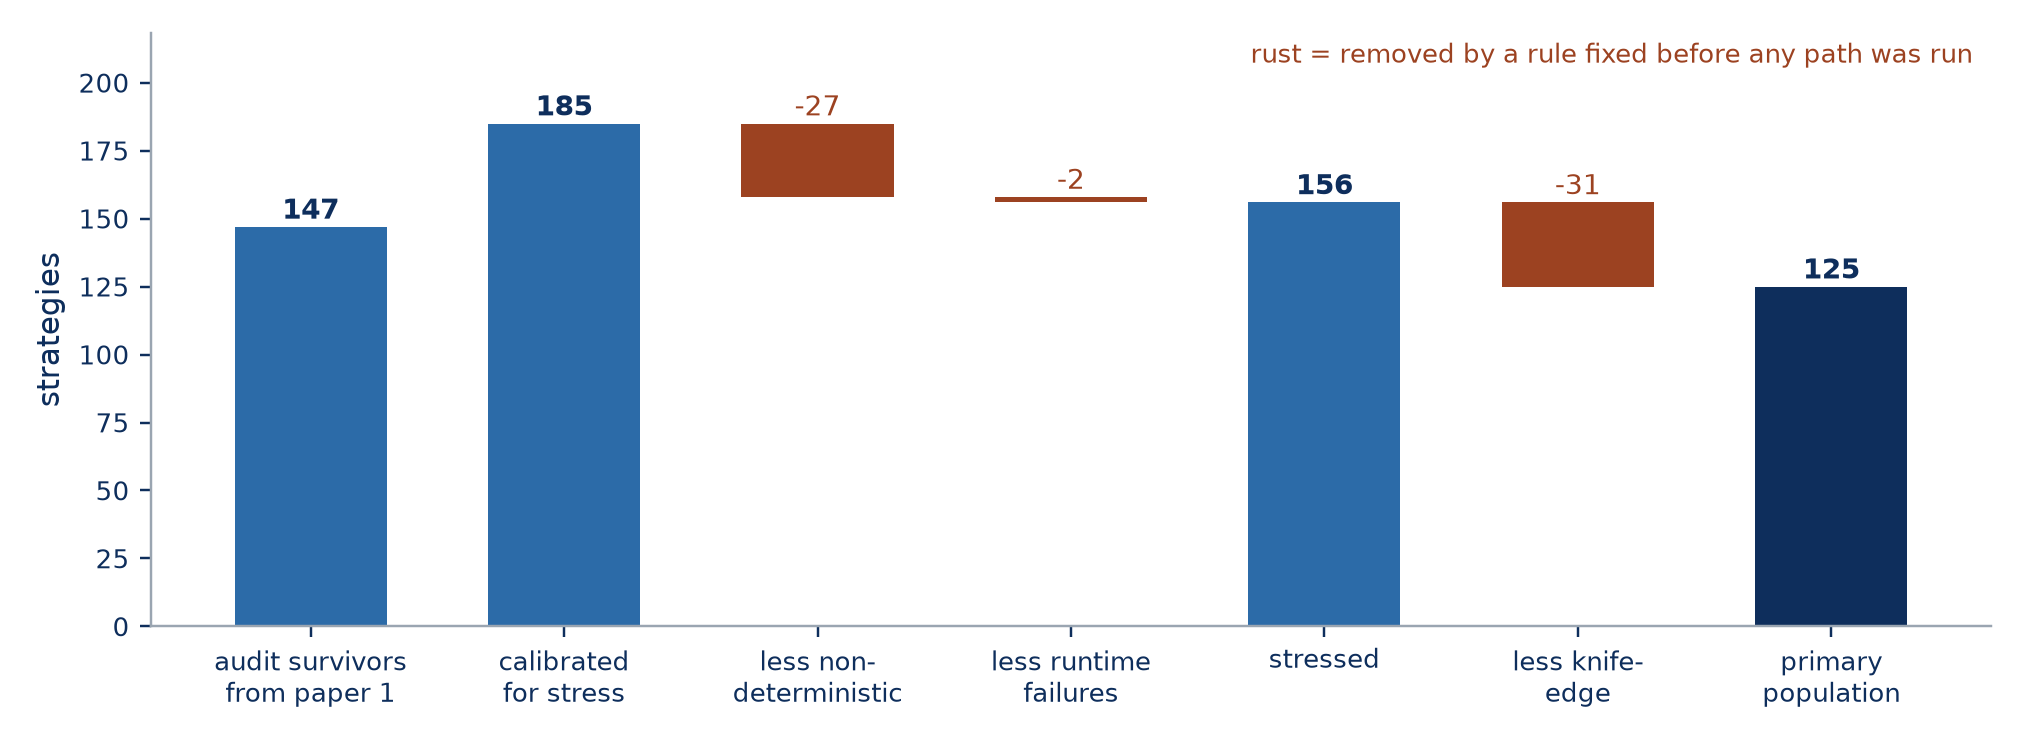
\includegraphics[width=\linewidth]{figures/fig_population_funnel.png}
\caption{From paper 1's audit survivors to the population this paper measures. The rise at the
second step is the standard academic factors joining as positive controls. Each rust bar is an
exclusion, each exclusion is non-random, and each is reported as a limitation in
\S\ref{sec:threats}. \textbf{Every rule that produced a rust bar was fixed before a single stress
path was run}, which is the only way an exclusion rule can be honest: applied afterwards, it is
indistinguishable from dropping the inconvenient cases.}
\label{fig:population}
\end{figure}


\subsection{Causal regime labelling}
\label{sec:regimes}

A hidden Markov model \citep{rabiner1989} over realised volatility, liquidity and macro state
labels each session with one of $K$ regimes. $K = \rsRegimeK{}$ was selected by BIC
\citep{schwarz1978} over \rsRegimeSelectionSessions{} sessions ending \rsRegimeSelectionEnd{} ---
\textbf{by information criterion, not by which labelling looked most recognisable}.

The labelling is \textbf{causal}. The model is refit on an expanding window
(\rsNRegimeRefits{} refits, from \rsRegimeTrainingSessionsFirst{} training sessions to
\rsRegimeTrainingSessionsLast{}) and decoded forward-only, so the label attached to a session uses
no information from after it. A full-sample fit would have been easier and is what the literature
usually does.

\begin{selfreport}[title={What causality costs, reported rather than smoothed}]
\textbf{\rsRegimeTerminalDisagreement\% of causal labels disagree with what the same estimator says
at the end of the sample}, and the labelling revises itself at a rate of
\rsRegimeRevisionRate\% as data arrives. That drift is not a defect to be tuned away --- it is what
it looks like to label regimes without hindsight, and a paper that reports clean stable labels has
probably used the future to get them. Regime occupancy ranges from \rsRegimeOccupancyMin{} to
\rsRegimeOccupancyMax{} sessions across the \rsRegimeK{} states, so no state is a degenerate corner.
\end{selfreport}

A hand-curated timeline of \rsNSebiEvents{} dated SEBI structural events ships beside the labels,
each with its source, so that a reader can check whether a labelled transition corresponds to
something that actually happened.

\subsection{Counterfactual Regime Resampling}
\label{sec:crr}

History supplied one path. \textbf{CRR manufactures more of them.}

The mechanism is a stationary block bootstrap \citep{politis1994} over \emph{dates}, conditioned on
regime label. Resampling dates rather than individual assets is what preserves the cross-sectional
correlation structure --- on any resampled day, every stock's return is the return it actually had
on some real day, so the relationships between them survive. Block length
\rsBlockLength{} sessions was selected by the automatic rule of \citet{politis2004}, as corrected
by \citet{patton2009}, at bandwidth \rsBlockBandwidth{}; blocks rather than individual days are
what preserve volatility clustering.

Conditioning on regime is what keeps a path plausible: a synthetic history is assembled from blocks
drawn within regime, so a calm stretch is built from calm days rather than from an arbitrary mix.
\rsCrrPaths{} paths over \rsCrrSessions{} sessions spanning \rsCrrWindowStart{} to
\rsCrrWindowEnd{}, at \rsCrrDrawSeconds{} seconds per draw.

\subsection{Validating the synthetic histories}
\label{sec:validation}

A resampler that produces statistically valid but economically absurd paths would invalidate
everything downstream, so the paths are tested rather than asserted. \rsNMoments{} target moments
--- volatility clustering, autocorrelation, skew and others --- are computed on the real series and
on each synthetic one, and the real value must fall plausibly inside the synthetic distribution.

\begin{finding}
\textbf{The conditional resampler fails \rsMomentsFailedConditional{} of \rsNMoments{} moments. The
unconditional one fails \rsMomentsFailedUnconditional{}}, with the real series sitting at the
\rsFailingMomentPercentile{}th percentile of the synthetic distribution on the failing moment.
Conditioning on regime is not a refinement --- it is the difference between paths that pass their
own validation and paths that do not.
\end{finding}

We report the unconditional failure rather than deleting the unconditional arm, and the
conditioning effect is itself measured: the two resamplers agree at Spearman
\rsConditioningEffectPaths{} on across-path fragility and \rsConditioningEffectRegimes{} on
across-regime fragility, so conditioning changes the level of the measurement more than it changes
the ordering.

\subsection{Two tiers, and two definitions of fragility}
\label{sec:definitions}

Fragility can be measured across two different kinds of environment variation, and the benchmark
computes both because they answer different questions.

\begin{itemize}
\item \textbf{Across regimes} --- how much does performance move between the
  \rsRegimeK{} labelled market states of the \emph{real} history? Cheap. The charter's primary
  definition.
\item \textbf{Across paths} --- how much does performance move between synthetic histories that
  never happened? Expensive: \rsTierOnePaths{} paths, \rsTierOneCpuHours{} CPU-hours,
  \rsTierOneSecondsPerPath{} seconds per path.
\end{itemize}

\textbf{These are not two estimates of one quantity.} They agree at Spearman
\rsDefinitionAgreement{} ($n=\rsTierAgreementN{}$), which is low enough that a paper reporting only
one of them under the unqualified word ``fragility'' would be making a choice it had not disclosed.
Both are reported throughout, and never pooled.

\subsection{Reproducibility}

Every number in this paper is generated from committed artefacts by a documented command sequence
and substituted into this document by macro. None is transcribed. The full pipeline runs from
\texttt{data/raw/} and writes a manifest per execution containing the git SHA, package versions,
model tags, seeds and input hashes. A cross-check on the warm-up window compared
\rsBurninCompared{} quantities and found \rsBurninBeyondTolerance{} beyond tolerance, with a worst
relative difference of $\rsBurninWorstRelative{}$.

% =====================================================================================
\section{Which shortcuts are safe}
\label{sec:tiers}

\begin{finding}
\tagmethod\ \ \textbf{A shortcut reproduced performance. It did not reproduce fragility.}
\end{finding}

\rsTierOneCpuHours{} CPU-hours is a lot for a measurement that a cheaper procedure might
approximate. The obvious shortcut is to skip re-simulating the strategy on each synthetic path and
instead resample the strategy's \emph{realised return series} directly --- vastly cheaper
(\rsTierTwoSeconds{} seconds for \rsTierTwoPaths{} paths, against
\rsTierOneSecondsPerPath{} seconds for one). Whether that is legitimate is an empirical question,
and we answered it by running the expensive version anyway and comparing.

\begin{figure}[t]\centering
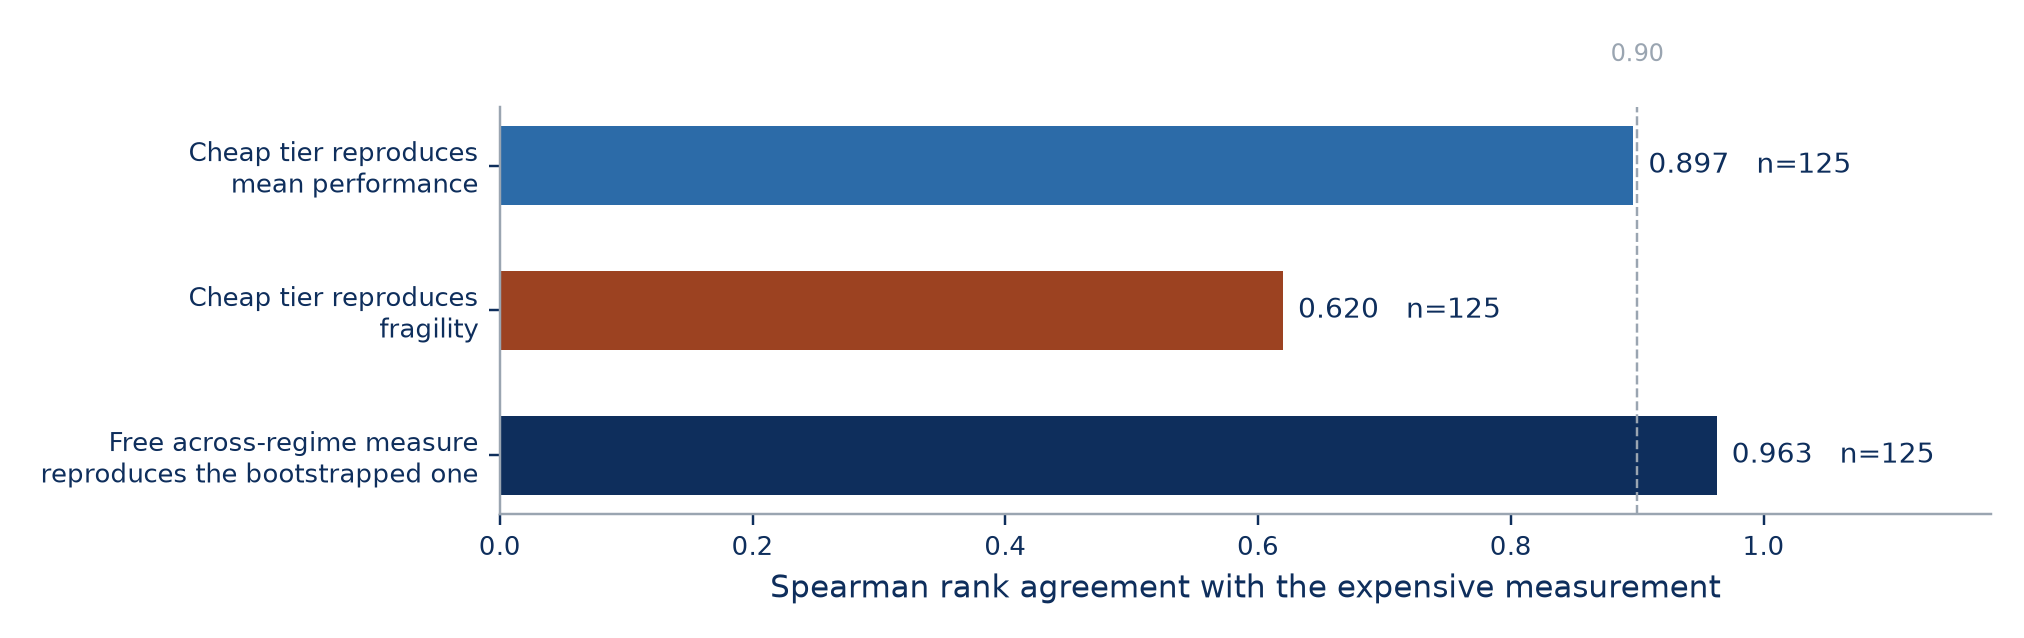
\includegraphics[width=\linewidth]{figures/fig_shortcut_safety.png}
\caption{Three shortcuts, measured against the expensive computation they would replace, on the
same strategies. Rank agreement, Spearman.}
\label{fig:shortcut}
\end{figure}

\takeaway{The cheap tier is an excellent proxy for \emph{how well a strategy does} and a poor proxy
for \emph{how much that varies}. Since the second is the entire point of the benchmark, the cheap
tier cannot replace the expensive one.}

\begin{table}[h]\centering\small
\caption{Cheap tier against full counterfactual re-simulation, $n=\rsTierAgreementN{}$.}
\label{tab:tiers}
\begin{tabular}{lrr}
\toprule
\thead{Quantity} & \thead{Rank agreement} & \thead{Median value} \\
\midrule
Mean performance & \rsTierAgreementMeanSharpe{} & --- \\
\textbf{Fragility} & \textbf{\rsTierAgreementFragility{}} &
  \rsTierMedianOne{} vs \rsTierMedianTwo{} \\
\bottomrule
\end{tabular}
\end{table}

\paragraph{What explains the divergence, and what we will not claim.} The two tiers differ in
exactly one respect: in the expensive tier the strategy \emph{re-decides} on the path it is given,
and in the cheap tier it cannot. The divergence is therefore \emph{consistent with} strategy
re-decision contributing materially to measured fragility --- and it is fragility rather than
performance that the cheap tier loses, which is what that explanation predicts.

\begin{scopebox}
\textbf{We do not claim causation from a rank correlation.} The observation is that two procedures
differing in one respect disagree on one quantity and agree on another. That is an empirical
methodological result with a practical consequence --- \emph{run the expensive tier} --- and it is
not a demonstration of the mechanism.
\end{scopebox}

\subsection{A shortcut that does hold}
\label{sec:shortcut}

Not every shortcut fails, and the benchmark distinguishes them by measurement rather than by
temperament. Across-regime fragility computed directly from a strategy's persisted return series
agrees with its bootstrapped counterpart at Spearman \rsShortcutSpearman{}
($n=\rsShortcutN{}$), with medians \rsShortcutMedianReal{} and \rsShortcutMedianBootstrap{}.

The expensive experiment was run in full and then used to \emph{validate} the free computation,
rather than being replaced by an assumption about it. Convergence in path count confirms the
expensive tier is itself converged: rank agreement against the full answer rises from
\rsConvergenceLow{} at \rsConvergenceLowPaths{} paths to \rsConvergenceAtHundred{} at
\rsTierOnePaths{} and \rsConvergenceHigh{} at \rsConvergenceHighPaths{}.

\takeaway{One shortcut is validated at \rsShortcutSpearman{} and adopted; another is measured at
\rsTierAgreementFragility{} and rejected. \textbf{Which is which was not predictable in advance},
and that is the argument for running both.}

% =====================================================================================
\section{Three properties of the population}
\label{sec:properties}

These are facts about the strategies and about the metric. They also appear in Threats to Validity,
because each limits what the rest of the paper can claim --- and they are stated here as well
because a reader who met them only among the caveats would reasonably conclude we had tried to keep
them quiet.

\subsection{A large minority of machine-written strategies are not deterministic}
\label{sec:nondeterminism}

\begin{finding}
\taglocal\ \ \textbf{\rsNNondeterministic{} of \rsNCalibrated{} strategies return a different result
when run twice on the same data with the same code}, with a worst-case Sharpe swing of
\rsWorstNondeterministicSwing{}. Every affected strategy is generator output. \textbf{Every
standard academic factor is deterministic.}
\end{finding}

This is a property of what the model wrote, not of the engine or the harness, and it has a direct
consequence for the whole enterprise: \textbf{a strategy whose score already varies for no reason
is arithmetically indistinguishable from one whose score varies because the market changed.}
Nondeterminism and fragility are the same measurement until the first is excluded.

The exclusion is non-random and we say so. The benchmark measures fragility on the subset of
machine-written strategies that happen to be reproducible, and reproducibility may correlate with
the simplicity that also drives fragility. The census was frozen before any stress path was run.

\subsection{The stability filter removes the fast end of the corpus}
\label{sec:knifeedge}

A strategy is \textbf{knife-edge} if its Sharpe ratio is not stable under a numerically negligible
change to its inputs --- a relative perturbation on the order of $10^{-15}$, which no economic
interpretation survives. \rsKnifeEdgeExcluded{} of \rsNStressed{} qualify, including
\rsKnifeEdgeFactors{} standard academic factor. The rule was applied without exemption.

\begin{figure}[h]\centering
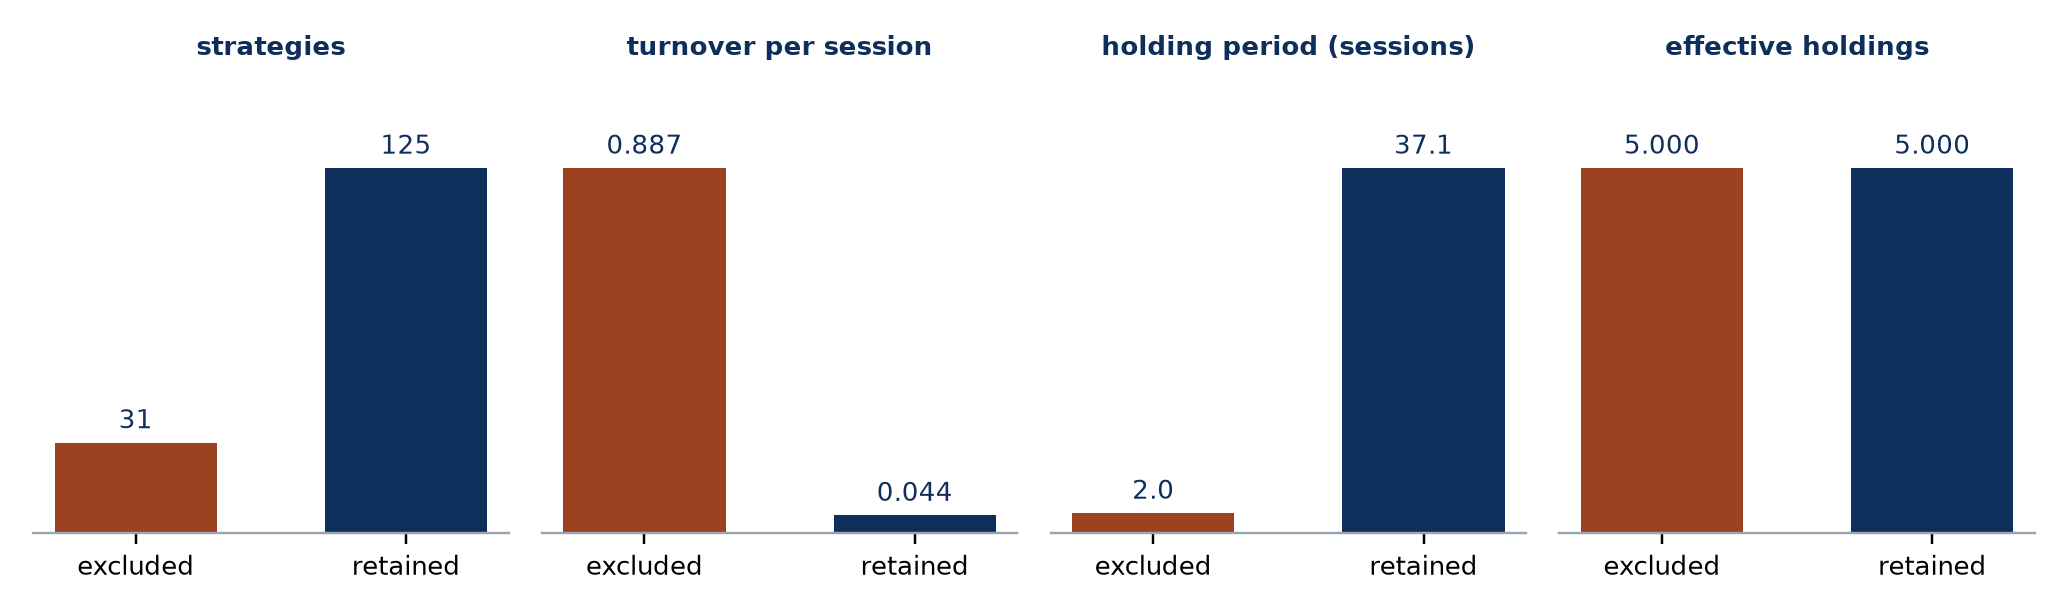
\includegraphics[width=\linewidth]{figures/fig_knife_edge.png}
\caption{How the knife-edge exclusions differ from the strategies that were retained, on four
characteristics with four different units. \textbf{The filter did not remove a random slice --- it
removed the fast end of the corpus}, and the paper's honesty depends on saying so, because the
retained population is therefore slower-trading than the one that entered.}
\label{fig:knifeedge}
\end{figure}


\begin{selfreport}[title={The exclusion is not random, and that is a limitation of every result
  downstream}]
The excluded strategies are systematically the \emph{fast} end of the corpus: twenty times the
turnover and a twentieth of the holding period of those retained. Every result downstream is
therefore conditioned on a restricted range of exactly the characteristic most likely to drive
fragility. Sharpe swing among the excluded has a median of \rsKnifeEdgeSwingMedian{} and a maximum
of \rsKnifeEdgeSwingMax{}, with \rsKnifeEdgeSwingAboveHalf{} above 0.5 --- so for most of them the
instability is small, and for a few it is not.
\end{selfreport}

\subsection{A strategy that is uniformly bad is measured as stable}
\label{sec:uniformlybad}

Fragility is a ratio with a mean in its denominator, and it scores consistency, not quality.
Nothing prevents a strategy that loses money in every regime from being uniformly consistent about
it.

\begin{finding}
\textbf{This is not hypothetical and it is not rare.} \rsUniformlyBadCount{} of \rsNPrimary{}
strategies have a negative Sharpe ratio in \emph{every} labelled regime. The most extreme,
\texttt{\rsUniformlyBadName}, ranges from \rsUniformlyBadWorstSharpe{} to
\rsUniformlyBadBestSharpe{} across the \rsRegimeK{} regimes --- and with a fragility of
\rsUniformlyBadFragility{} it ranks \rsUniformlyBadRank{} of \rsNPrimary{} on the low-fragility end
of the corpus. \textbf{It is among the most robust strategies we measured, and it never makes
money.}
\end{finding}

\textbf{A fragility score is therefore uninterpretable without a performance figure beside it}, and
must never be used as a standalone ranking. Our own narrative layer does not enforce this and
describes one such strategy as most reliable in a regime in which it loses money
(\S\ref{sec:narratives}). A further \rsNNearZeroMean{} strategies are flagged because a near-zero
mean in the denominator inflates the ratio for arithmetic reasons; how many sit close enough to
that boundary for the flag to miss them is unknown.

% =====================================================================================
\section{Predicting fragility, and why it fails}
\label{sec:prediction}

The benchmark's first task: predict a strategy's fragility from its characteristics alone ---
turnover, holding period, concentration, book-similarity decay, and factor exposures obtained from
one joint regression on all \rsFactorCount{} factors at once --- \emph{without running the stress
suite}. If that worked it would be genuinely useful, since the stress suite costs
\rsTierOneCpuHours{} CPU-hours and the characteristics are free.

\subsection{It does not work}

\begin{figure}[t]\centering
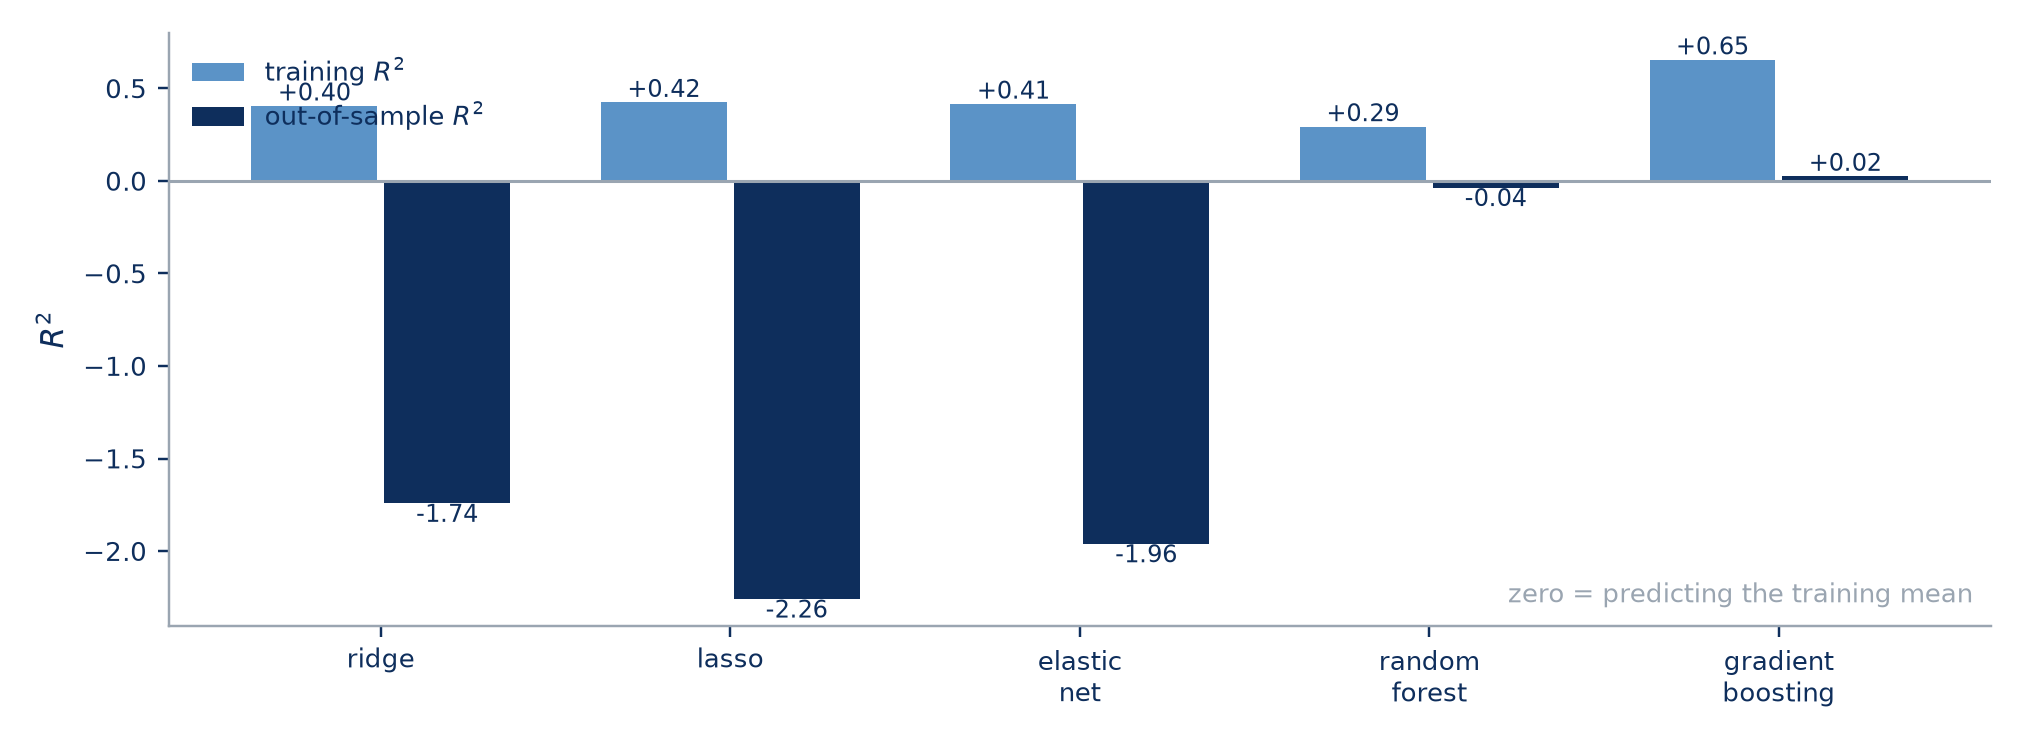
\includegraphics[width=\linewidth]{figures/fig_predictor_gap.png}
\caption{Five model families on identical folds, $n=\rsPredictorRows{}$. Training against
out-of-sample $R^2$ on the primary target. Zero is what predicting the training mean scores.}
\label{fig:predictorgap}
\end{figure}

\takeaway{Every model fits its training folds far better than it generalises, and the gap is
\emph{widest} for the model with the most capacity. That is the signature of variance rather than
bias --- which is why we added no capacity, and why a larger corpus rather than a larger model is
the correct next experiment.}

\rsPredictorRows{} strategies, \rsPredictorFeatures{} features, five model families on identical
folds.

Figure~\ref{fig:predictorgap} carries all ten figures. The gap between the paired bars is the
diagnosis, and it is why we report the null as a property of the sample rather than of the model
family.


\takeaway{The best out-of-sample $R^2$ is \rsPathsRawBestRsquared{}, from
\rsPathsRawBestRsquaredModel{} \citep{breiman2001}. Predicting the training mean would score zero.
This is not a model that needs tuning; it is a problem that is not solvable at this sample size.}

\subsection{The diagnosis: variance, not bias}

Reporting a null without diagnosing it is not useful, because the reader cannot tell whether to try
harder or to stop. We separate the candidate explanations by measurement.

\begin{table}[h]\centering\small
\caption{Candidate explanations for the null, each measured.}
\label{tab:diagnosis}
\begin{tabular}{p{0.27\linewidth}p{0.30\linewidth}p{0.36\linewidth}}
\toprule
\thead{Explanation} & \thead{Measurement} & \thead{Verdict} \\
\midrule
Heavy-tailed target &
Skew \rsPathsRawSkew{}, kurtosis \rsPathsRawKurtosis{}; top 5\% of observations hold
\rsPathsRawTailShareFive\% of the variance &
Real. A $\log(1+x)$ transform lifts the best $R^2$ to \rsPathsLogBestRsquared{} --- still weak. \\
\midrule
Multicollinear features &
Condition number \rsFeatureCondition{}; worst pair \texttt{\rsFeatureWorstPairA} and
\texttt{\rsFeatureWorstPairB} at $r=\rsFeatureWorstPairR{}$ &
Present, and it degrades the linear models specifically. \\
\midrule
Influential observations &
Dropping the 5 most influential moves $R^2$ by \rsPathsRawBoostingDropFive{}; the 10 most, by
\rsPathsRawBoostingDropTen{} \citep{cook1977} &
Severe. The result is not stable to a handful of rows. \\
\midrule
Too few strategies &
Learning curve: \rsPathsRawCurveAtForty{} at \rsCurveSizeAtForty{} rows,
\rsPathsRawCurveAtHundred{} at \rsCurveSizeAtHundred{} &
\textbf{Still climbing at the full sample.} More data would help; more capacity would not. \\
\midrule
No relationship at all &
Permutation test, \rsPermutations{} shuffles \citep{ojala2010}:
$p=\rsPathsRawPermPSpearman{}$ on rank, $p=\rsPathsRawPermPRsquared{}$ on level &
\textbf{Rejected for ranking, not rejected for level.} \\
\bottomrule
\end{tabular}
\end{table}

\begin{finding}
\textbf{Strategy characteristics contain statistically detectable \emph{ranking} information and
very weak information about the \emph{level} of fragility.} The permutation test rejects the null
for rank order ($p=\rsRegimesLogPermPSpearman{}$--$\rsPathsRawPermPSpearman{}$) while failing to
reject it for the level on three of four targets.
\end{finding}

\textbf{Every model fits its training folds far better than it generalises, and the gap is widest
for the model with the most capacity} --- gradient boosting at \rsPathsRawBoostingGap{} against
the random forest's \rsPathsRawForestGap{}. That is the signature of variance rather than bias.
\textbf{We therefore added no capacity}, which is the action the diagnosis implies and the opposite
of what a search for a better number would have produced.

The five characteristics that carry the most weight, reported for completeness rather than as an
economic finding: \texttt{\rsImportanceFirstName} (\rsImportanceFirstValue),
\texttt{\rsImportanceSecondName} (\rsImportanceSecondValue),
\texttt{\rsImportanceThirdName} (\rsImportanceThirdValue),
\texttt{\rsImportanceFourthName} (\rsImportanceFourthValue) and
\texttt{\rsImportanceFifthName} (\rsImportanceFifthValue).

% =====================================================================================
\section{Two corrections, reported as findings}
\label{sec:corrections}

\begin{selfreport}[title={Our first answer was better, and wrong}]
The first version of the fragility predictor produced a modest positive result. It was wrong, and
we found out by deduplicating the corpus.

\textbf{Correction 1 --- duplicate leakage.} \rsDuplicateClusters{} clusters of strategies produce
\emph{identical} realised return series, covering \rsDuplicateMembers{} of
\rsDuplicateCompared{} compared strategies, with a largest cluster of
\rsLargestDuplicateCluster{}. A duplicate sitting in a training fold with its twin in the test fold
is not generalisation --- it is memorisation with the answer key in the room. Deduplicating
(\rsDuplicateRemoved{} rows removed, \rsDuplicateUncompared{} not comparable) moved the Spearman
result from \rsLeakageWithDuplicates{} at $n=\rsLeakageNWith{}$ to
\rsLeakageWithoutDuplicates{} at $n=\rsLeakageNWithout{}$. \textbf{The duplicates were worth
\rsLeakageDelta{} of $R^2$}, which is to say: the entire original result.

\textbf{Correction 2 --- a duplicated feature.} One feature column duplicated another under a
different name, inflating that characteristic's apparent importance.

Both corrections made every reported number worse. Both are in the benchmark's corrections log.
And the duplicate structure ships as a benchmark artefact rather than being quietly removed,
because \textbf{it is a fact about machine-written strategy corpora, not a blemish on ours} --- a
near-duplicate rule at threshold \rsNearDuplicateThreshold{} fires a further
\rsNearDuplicatePairs{} times below the exact criterion.
\end{selfreport}

% =====================================================================================
\section{Stress narratives}
\label{sec:narratives}

A local model (\rsNarrativeModel) generates natural-language descriptions of when a strategy
fails --- the explainability layer that would make a fragility number presentable to a risk
committee. \rsNarrativeCount{} narratives at \rsNarrativeSeconds{} seconds each.

\begin{scopebox}
\textbf{The narrative layer is the least validated component in this paper and we do not recommend
relying on it.} It reads a fragility score and a set of regime performances and produces fluent
prose about them; nothing checks that the prose is warranted. It described one of the
\rsUniformlyBadCount{} uniformly-losing strategies of \S\ref{sec:uniformlybad} as most reliable in
a regime in which it loses money. That sentence is true about consistency and misleading about
everything a reader would take from it.
\end{scopebox}

% =====================================================================================
\section{Does any of this depend on who wrote the strategies?}
\label{sec:generators}

Everything above was measured on a corpus written by one local seven-billion-parameter model. The
objection is obvious and it is the right one to raise: this paper may be describing that model
rather than machine-written strategies in general.

So the identical frozen task specification was issued to \rsGvArms{} frontier models
(\rsGvRequestsPerArm{} independent requests each) and all \rsGvTotal{} strategies were passed
through this benchmark \textbf{with no parameter altered and no line of measurement code added}.
The same benchmark was separately applied to \pgmParadigmArms{} generation methods on the local
model.

\begin{figure}[t]\centering
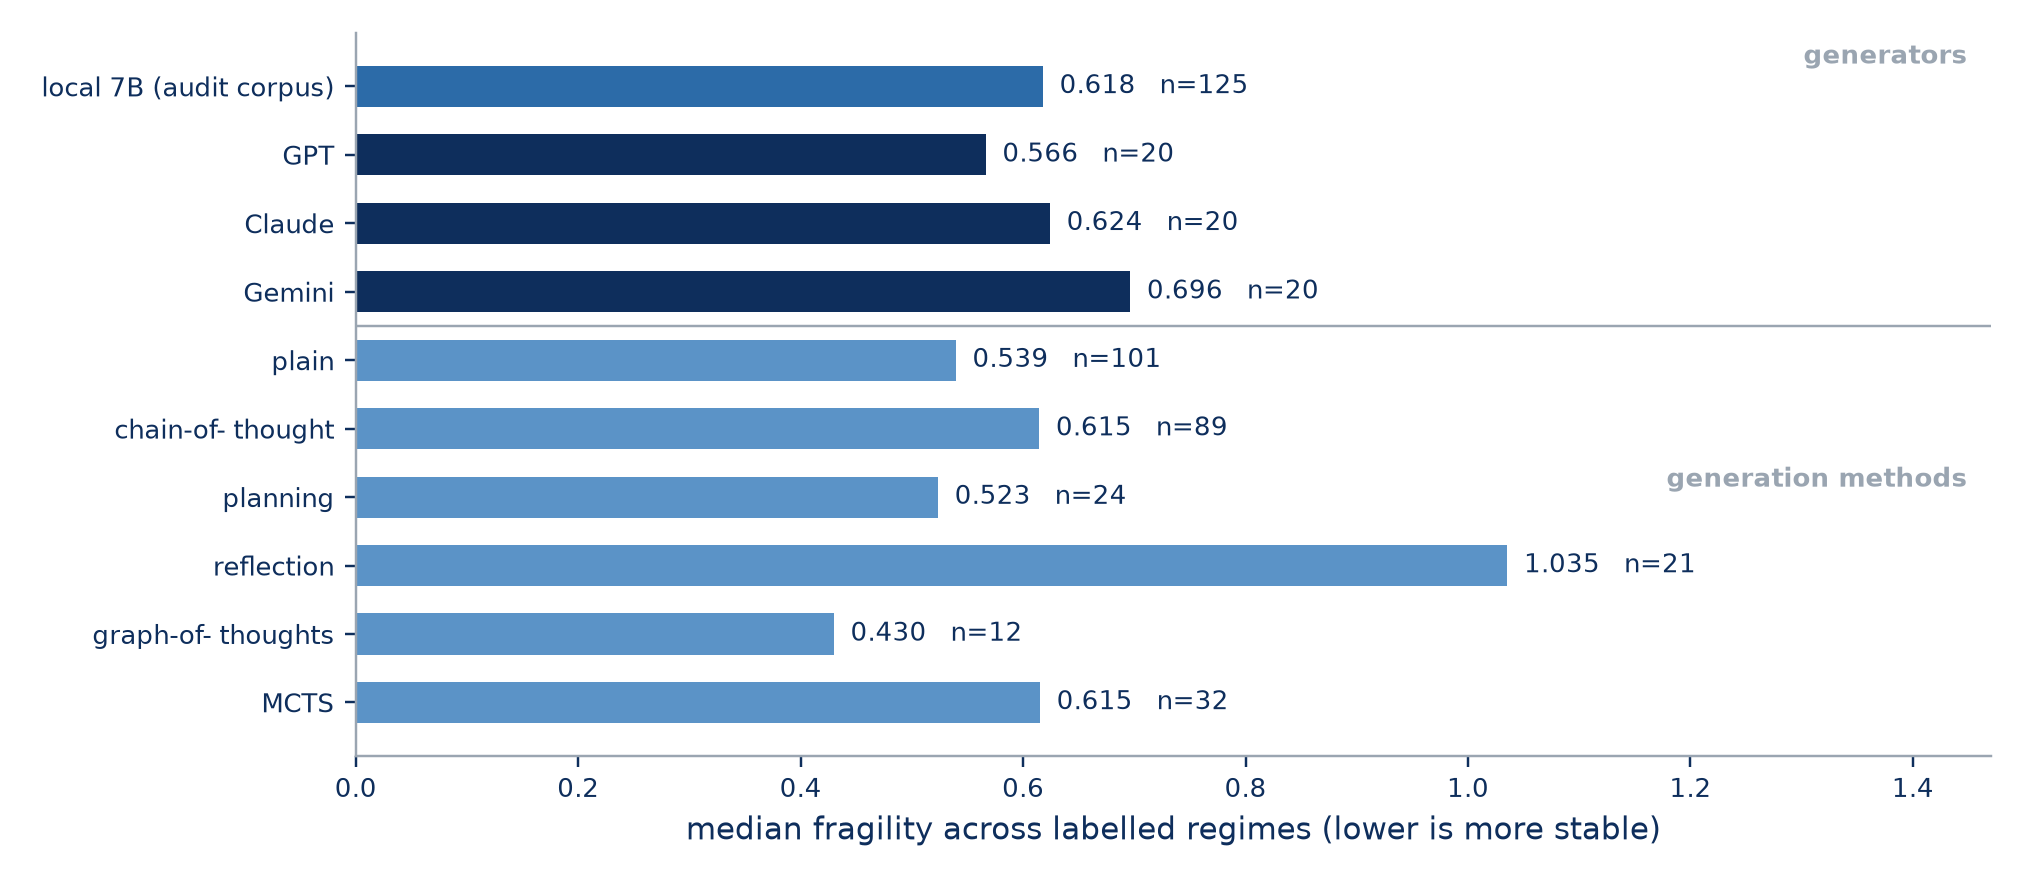
\includegraphics[width=\linewidth]{figures/fig_fragility_by_origin.png}
\caption{Median fragility across labelled regimes --- one definition, one axis. The upper block
varies \emph{who} wrote the strategy; the lower block varies \emph{how} the same model was
prompted. Sample sizes are printed on every bar because they vary by an order of magnitude.}
\label{fig:origin}
\end{figure}

\takeaway{Fragility does not move much with the generator, and does not move much with the
generation method either. It is closer to a property of the market than of the author.}

\subsection{Fragility is generator-independent}

\begin{figure}[t]\centering
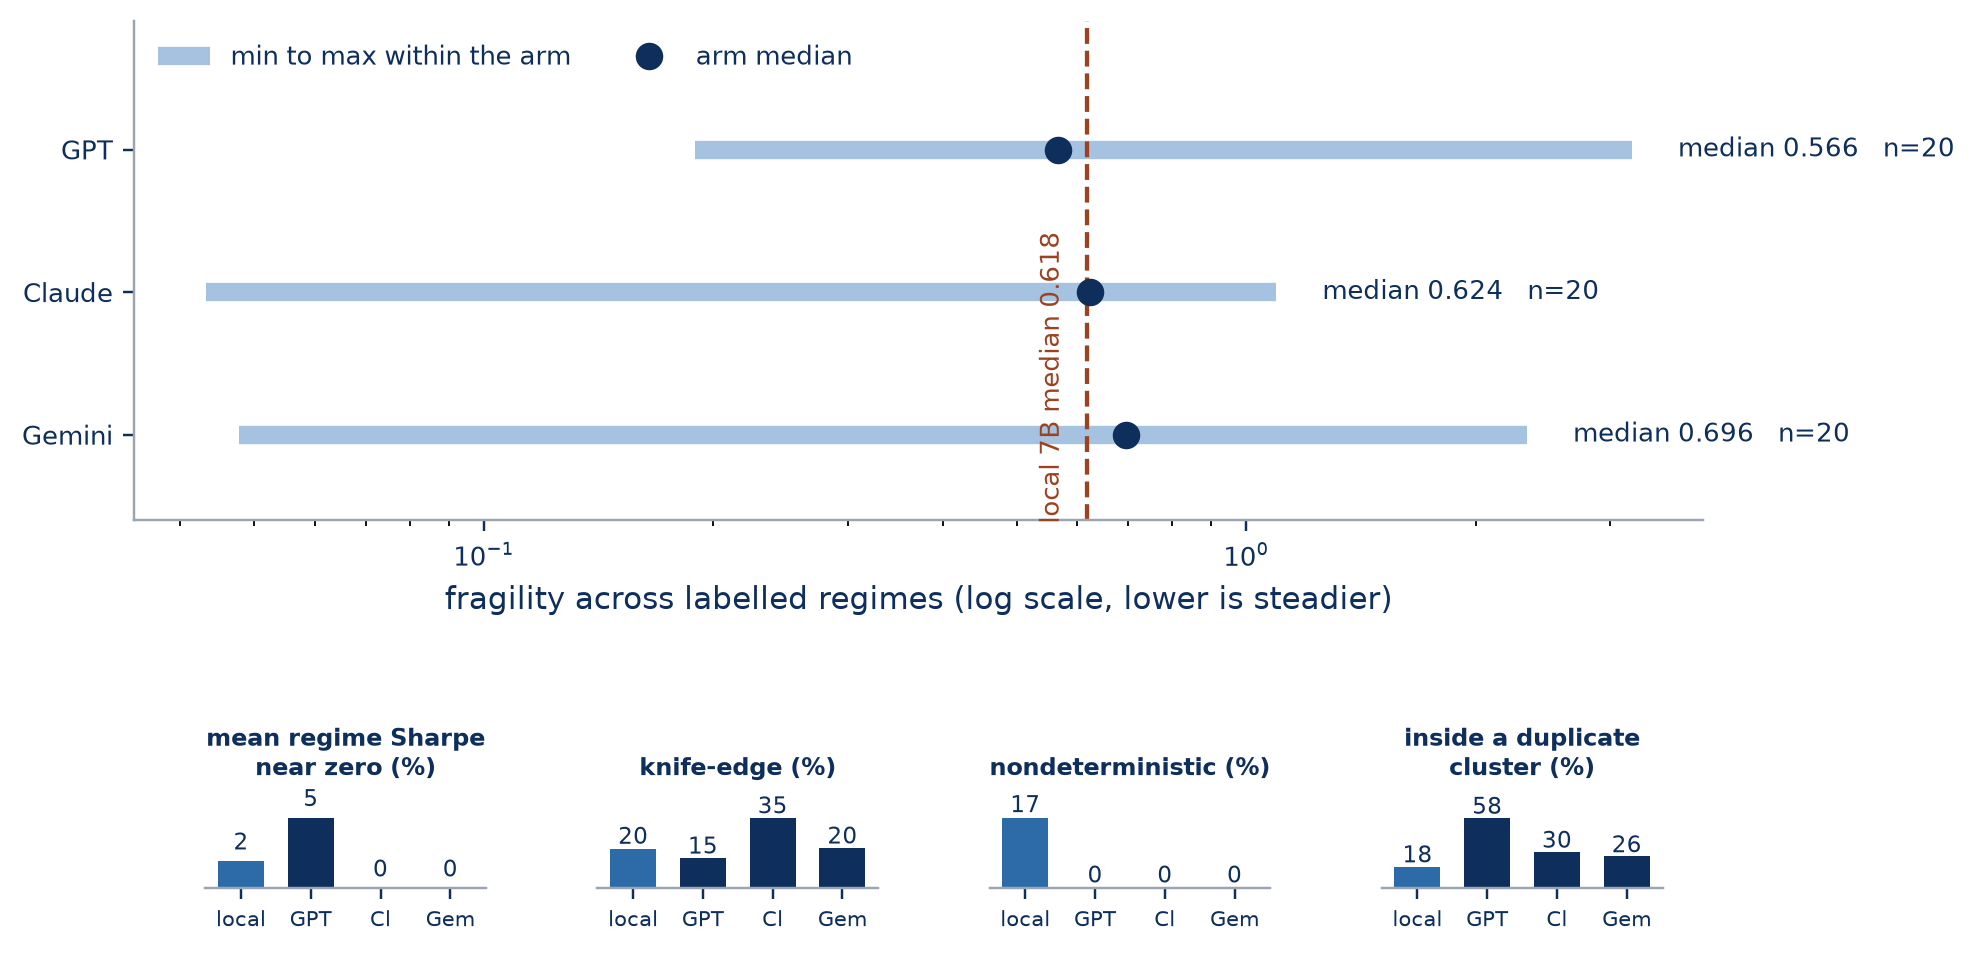
\includegraphics[width=\linewidth]{figures/fig_generator_fragility_range.png}
\caption{Every RegimeStress measurement, by generator. \emph{Upper:} fragility across labelled
regimes --- the charter's primary definition --- with the full range each median summarises, on a
log axis. \textbf{The spread inside any one arm is far wider than the gap between arms.}
\emph{Lower:} the three pathologies and the duplicate structure, as rates so that a
\rsGvGptN{}-strategy arm and the \rsNStressed{}-strategy local corpus sit on one scale.
\texttt{Cl} is Claude and \texttt{Gem} is Gemini.}
\label{fig:generators}
\end{figure}


\begin{finding}
\tagindep\ \ \textbf{Fragility is a property of the market, not of the author.} The primary measure
is \rsGvLocalRegimeMedian{} on the local corpus against \rsGvGptRegimeMedian{},
\rsGvClaudeRegimeMedian{} and \rsGvGeminiRegimeMedian{} on the three frontier arms.
\textbf{Every arm lands within a sixth of the local median.} This is the result the benchmark most
needed and did not have: what it measures survives a change of generator.
\end{finding}

\subsection{The knife edge recurs; nondeterminism does not}

Between fifteen and thirty-five per cent of each frontier arm sits on a knife edge, against
\rsNKnifeEdge{} of \rsNStressed{} locally. The worst frontier case moves by more than two Sharpe
units under a fifteenth-decimal-place perturbation. \S\ref{sec:knifeedge} argued this is a property
of how strategies are written rather than of any one writer, and the frontier arms support that.

\begin{finding}
\tagfrontier\ \ \textbf{Nondeterminism does not recur.} Not one of the \rsGvTotal{} frontier
strategies changes its result across two hash seeds or across a replicate at a fixed seed, against
\rsNExcludedNondeterministic{} of \rsNStressed{} locally. Iterating an unordered container is a
habit the frontier models do not have. \textbf{It is the one measured pathology in this paper that
is genuinely a property of the generator}, and it is the reason \S\ref{sec:nondeterminism}'s
exclusion is a statement about the local model rather than about machine-written code.
\end{finding}

\subsection{The predictor's failure is not local either}

\S\ref{sec:prediction} reported that fragility cannot be predicted from strategy characteristics.
Trained unchanged on the same \rsGvPredTrainN{} local strategies and applied to the
\rsGvPredPooledN{} frontier strategies as held-out data, the model reaches a pooled out-of-sample
$R^2$ of \rsGvPredPooledRsq{} against its training mean: \textbf{no better than a constant, on data
from a different generator.} The negative result is a property of the problem.

\begin{scopebox}
One caveat we did not expect, reported as \textbf{exploratory} since it appears in no
pre-registration: while the level predictions are worthless, the rank ordering is not. Spearman
correlation between predicted and measured fragility is \rsGvGptPredSpearman{},
\rsGvClaudePredSpearman{} and \rsGvGeminiPredSpearman{} on the three arms and
\rsGvPredPooledSpearman{} pooled. The model cannot say how fragile a strategy is; it partially
orders which of two is more fragile. \textbf{At \rsGvGptN{} strategies per arm this is a direction
worth testing properly, not a finding.}
\end{scopebox}

\subsection{Duplicate clustering persists everywhere}

\rsGvGptDupCovered{} of \rsGvGptDupCompared{} comparable GPT strategies sit inside an
exact-duplicate cluster, \rsGvClaudeDupCovered{} of \rsGvClaudeDupCompared{} on Claude and
\rsGvGeminiDupCovered{} of \rsGvGeminiDupCompared{} on Gemini --- across requests issued in
independent sessions. The near-duplicate rule that the exact criterion does not merge fires
\rsGvClaudeNearPairs{} times on Claude and \rsGvGptNearPairs{} and \rsGvGeminiNearPairs{} times on
the other two.

\textbf{The redundancy finding of \S\ref{sec:corrections} holds at the frontier.} Paper 1 reports
the sharper version of this: strategies from two \emph{different vendors} whose realised return
series are identical to floating-point precision.

\subsection{Does the generation \emph{method} change fragility?}

The same benchmark, applied to \pgmParadigmArms{} generation methods on the local model, all using
the across-regime definition.

The lower block of Figure~\ref{fig:origin} carries the six arms on the same axis and the same
definition as the upper block, so the two questions --- does the generator matter, does the method
matter --- can be read against one another without rescaling.


\takeaway{Reflection is the outlier at \pgmReflectFrag{} on \pgmReflectFragN{} strategies --- the
only method whose median exceeds one, meaning its strategies' performance varies by more than its
own average
size. Every other method sits in a band from \pgmGraphFrag{} to \pgmCotFrag{}. We report the
reflection figure without an explanation for it.}

\begin{scopebox}
\textbf{These are not comparable to the tier-1 across-path figures}, which on the same frontier
arms are \rsGvGptFragMedian{} for GPT (range \rsGvGptFragMin{}--\rsGvGptFragMax{}),
\rsGvClaudeFragMedian{} for Claude (\rsGvClaudeFragMin{}--\rsGvClaudeFragMax{}) and
\rsGvGeminiFragMedian{} for Gemini (\rsGvGeminiFragMin{}--\rsGvGeminiFragMax{}). The two
definitions must never be plotted on one axis. \S\ref{sec:definitions} measured their agreement at
\rsDefinitionAgreement{} ($n=\rsTierAgreementN{}$), which is too low for one to stand in for the
other. Every arm in both blocks of Figure~\ref{fig:origin} is an across-regime figure, matching the
upper panel of Figure~\ref{fig:generators} and nothing else in this paper.

\textbf{Nor is the local reference in the two blocks the same population.}
Figure~\ref{fig:generators} uses paper 1's pooled audit corpus ($n=\rsGvLocalRegimeN{}$);
the plain-prompting arm in Figure~\ref{fig:origin}'s lower block is a separate
\pgmPlainDraws{}-draw arm generated for the methodology experiment ($n=\pgmPlainFragN{}$). They are
two samples from the same generator under the same prompt, and their medians differ.
\end{scopebox}

% =====================================================================================
\section{The standard-factor control, and a reversal}
\label{sec:factors}

\begin{finding}
\tagexpl\ \ \textbf{The published factors are \emph{more} fragile than the machine-written corpus}
--- median \sfMedFrag{} across regimes against \rsGvLocalRegimeMedian{}
($n=\sfN{}$ against $n=\rsGvLocalRegimeN{}$). The metric runs backwards from the direction anyone
would predict, and the reason is \S\ref{sec:uniformlybad}.
\end{finding}

\S\ref{sec:generators} varied the generator. This section varies something else: the population
includes \sfN{} standard factor strategies --- momentum, low volatility, short-term and long-term
reversal, relative strength, an equal-weight market reference, and two deliberate controls. They
are published, long-standing, and were never drawn from any search of ours.

\begin{figure}[h]\centering
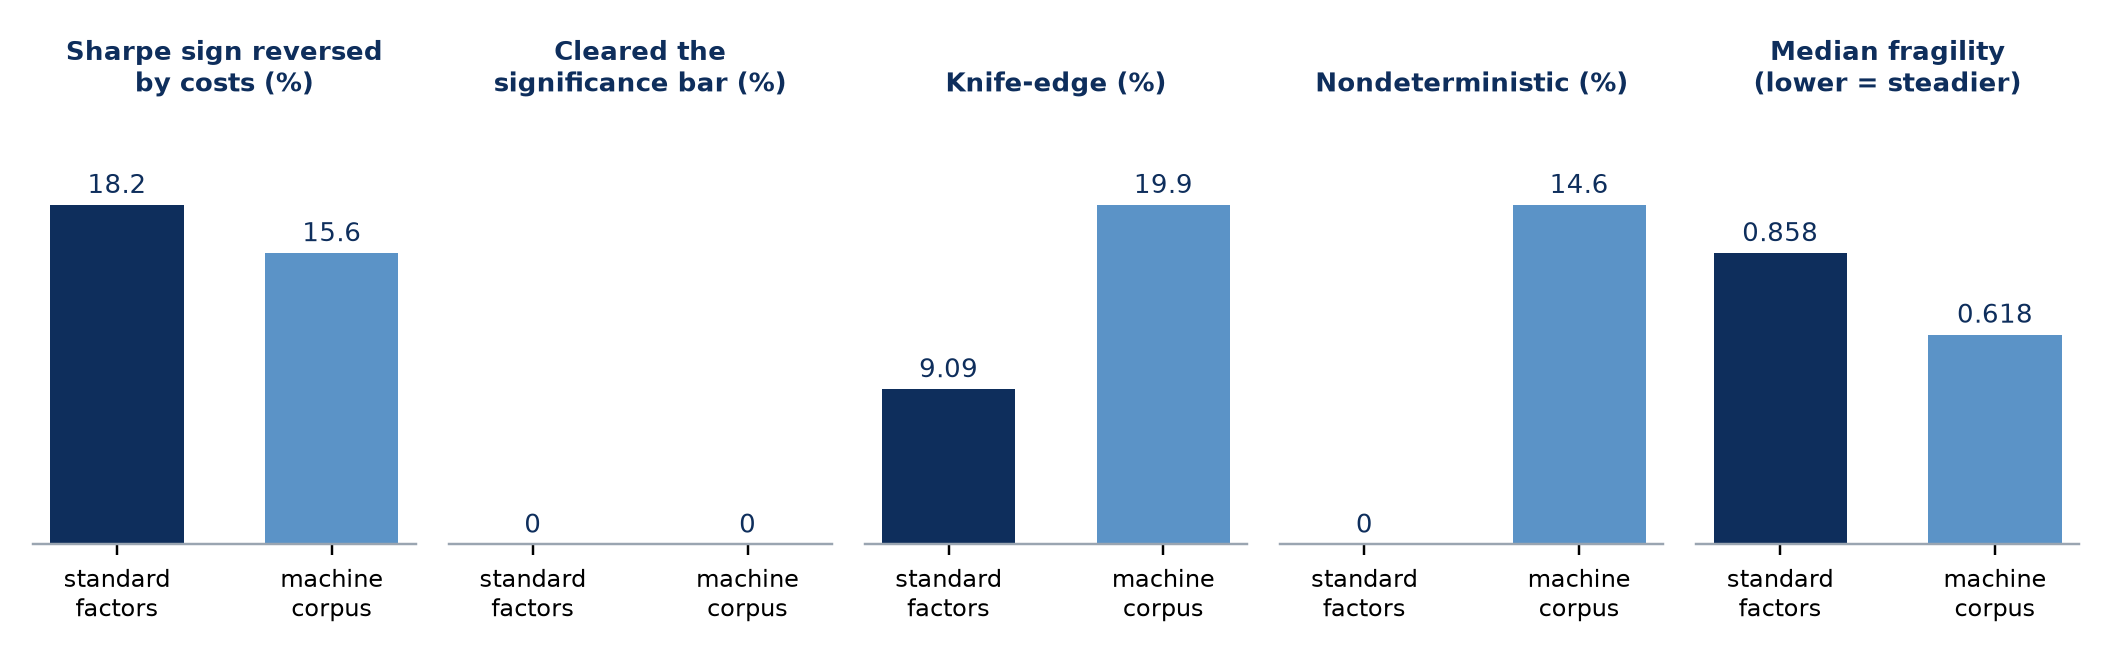
\includegraphics[width=\linewidth]{figures/fig_factors_vs_corpus.png}
\caption{The standard-factor arm beside the machine-written corpus on five frozen tests, each
panel on its own scale because the five quantities share no unit. Sample sizes differ by an order
of magnitude --- \sfN{} against \rsNStressed{} --- and the two reversals, costs and fragility
running opposite ways, are the reason this is drawn rather than tabulated.}
\label{fig:factorsvscorpus}
\end{figure}


\paragraph{Why fragility runs backwards, and why that is the metric's fault rather than the
corpus's.} A published factor takes real positions and its performance genuinely differs between a
crisis and a calm stretch --- which is what fragility is supposed to measure. Much of the machine
corpus is near-flat or uniformly mediocre, and a strategy that does approximately nothing does
approximately the same nothing in every regime. It therefore scores as admirably stable.
\S\ref{sec:uniformlybad} showed \rsUniformlyBadCount{} of \rsNPrimary{} machine strategies losing
money in \emph{every} regime, one of them ranking \rsUniformlyBadRank{} of \rsNPrimary{} for
robustness.

\begin{finding}
\textbf{The standard-factor arm converts that from an argument into a measurement.} A population
known in advance to contain real strategies scores \emph{worse} on our fragility metric than a
population known to be mostly inert. \textbf{Any use of fragility as a standalone ranking would
have preferred the inert one.} The metric is not wrong; it answers a question about consistency and
we must stop reading it as a question about quality.
\end{finding}

\paragraph{Nondeterminism is the one clean separation.} \sfNondet{} of \sfN{} standard factors are
nondeterministic, against \rsNExcludedNondeterministic{} of \rsNStressed{} machine-written
strategies and \rsGvGptNondeterministic{} of \rsGvTotal{} frontier ones. Combined with
\S\ref{sec:generators}, the picture is consistent: nondeterminism is a habit of one small model,
absent from published code and absent from frontier output.

\begin{scopebox}
\textbf{Eleven strategies.} Every rate here has a denominator of eleven, so one strategy moves it
by nine points. The arm is a control, not a sample. \textbf{It is also not a ``human versus AI''
comparison}: the contrast is \emph{published and long-standing} against \emph{machine-written}, and
these fixtures were hand-written for a different purpose by an author who knew the evaluation.
The deflation column and this assembly appear in no pre-registration and are exploratory.
\end{scopebox}

% =====================================================================================
\section{Design flaws, mistakes, and things that did not work}
\label{sec:flaws}

\begin{table}[h]\centering\small
\caption{Defects in our own apparatus and results that failed, with what each cost.}
\label{tab:flaws}
\begin{tabular}{p{0.28\linewidth}p{0.42\linewidth}p{0.22\linewidth}}
\toprule
\thead{Defect or null} & \thead{What it cost} & \thead{Where} \\
\midrule
Duplicate leakage &
\rsDuplicateClusters{} clusters of identical return series split across training and test folds
were worth \rsLeakageDelta{} of $R^2$ --- the whole of our original positive result. &
\S\ref{sec:corrections} \\
\midrule
A duplicated feature column &
One characteristic appeared twice under different names, inflating its apparent importance. &
\S\ref{sec:corrections} \\
\midrule
Fragility scores consistency, not quality &
A strategy losing money in every regime ranks \rsUniformlyBadRank{} of \rsNPrimary{} for
robustness. Now measured against a control arm that scores \emph{worse} than the inert corpus. &
\S\ref{sec:uniformlybad}, \S\ref{sec:factors} \\
\midrule
Both exclusions are non-random &
Knife-edge removes the fast end of the corpus (turnover \rsKnifeEdgeTurnoverExcluded{} against
\rsKnifeEdgeTurnoverRetained{}); nondeterminism removes a
subset that may differ systematically. Every result is conditioned on a restricted population. &
\S\ref{sec:properties} \\
\midrule
The narrative layer is unvalidated &
It described a money-losing strategy as most reliable in a regime where it loses money. We do not
recommend relying on it. & \S\ref{sec:narratives} \\
\midrule
Regime labels drift &
\rsRegimeTerminalDisagreement\% disagree with the terminal fit. The honest cost of refusing
hindsight, and it means the partition itself is uncertain. & \S\ref{sec:regimes} \\
\midrule
Synthetic histories are an assumption &
Every across-path number inherits it. \rsMomentsFailedConditional{} moment failures of
\rsNMoments{} is the strongest evidence we can offer and is not the same as being right. &
\S\ref{sec:threats} \\
\bottomrule
\end{tabular}
\end{table}

\subsection{Results that failed}

\begin{itemize}
\item \textbf{Fragility cannot be predicted from strategy characteristics.} $R^2 =
  \rsPathsRawBestRsquared{}$ at $n=\rsPredictorRows{}$, and \rsGvPredPooledRsq{} on frontier
  strategies as held-out data. This was the benchmark's first task.
\item \textbf{The cheap stress tier cannot replace the expensive one} for the quantity of interest:
  \rsTierAgreementFragility{} on fragility against \rsTierAgreementMeanSharpe{} on performance.
\item \textbf{Our first predictor result was better and wrong}, by \rsLeakageDelta{} of $R^2$.
\item \textbf{Fragility does not separate generators} --- which we report as a success for the
  benchmark and a null for anyone hoping to rank models by it.
\item \textbf{Our own metric prefers strategies that do nothing}, demonstrated in
  \S\ref{sec:factors} on a control population.
\end{itemize}

% =====================================================================================
\section{Threats to validity}
\label{sec:threats}

These are the reasons a reader should discount what is above. They are a section rather than a
footnote because several are load-bearing.

\paragraph{T1 --- The synthetic histories are an assumption, not evidence.} Across-path fragility
rests entirely on the resampler being a reasonable model of how markets could have gone. It passes
\rsMomentsFailedConditional{} failures on \rsNMoments{} moments, which is the strongest evidence we
can offer and is not the same as being right. \textbf{This is the paper's single largest
assumption} and every across-path number inherits it.

\paragraph{T2 --- Both exclusions are non-random.} Knife-edge exclusion removes the fast end of the
corpus (\S\ref{sec:knifeedge}); nondeterminism exclusion removes strategies that may differ
systematically from those retained (\S\ref{sec:nondeterminism}). Every downstream result is
conditioned on a restricted population.

\paragraph{T3 --- The regime labels drift.} \rsRegimeTerminalDisagreement\% of causal labels
disagree with the terminal fit. That is the honest cost of not using the future, and it means the
regime partition a strategy is scored against is itself uncertain.

\paragraph{T4 --- Sample size bounds the prediction task, and we know it does.} The learning curve
is still climbing at \rsCurveSizeAtHundred{} rows. A larger corpus is the correct next experiment,
and it is not one we can run under this programme's constraints.

\paragraph{T5 --- Fragility scores consistency, not quality.} \S\ref{sec:uniformlybad}. Any use of
these numbers as a standalone ranking is a misuse, including by our own narrative layer.

\paragraph{T6 --- One market, one window, one corpus.} \rsCrrWindowStart{} to
\rsCrrWindowEnd{}, Indian large-cap equities, a corpus of machine-written strategies. Factor
exposures are computed against \rsFactorCount{} factors with a design condition number of
\rsFactorCondition{} and a worst pair correlation of \rsFactorWorstPair{}, so the exposures are not
cleanly separated from one another.

\paragraph{T7 --- The frontier arms are \rsGvGptN{} strategies each.} Every claim in
\S\ref{sec:generators} rests on \rsGvTotal{} strategies in total. They are enough to show that
fragility does not move dramatically with the generator; they are not enough to establish that it
does not move at all.

% =====================================================================================
\section{What this tells us about AI-driven research}
\label{sec:meaning}

Three claims, at three scopes, kept separate.

\paragraph{Generator-independent \tagindep} Fragility itself, the fragility-prediction null, and
the knife-edge pathology all reproduce across four generators. These are the claims that license
the benchmark being used by other people.

\paragraph{Generator-specific \taglocal} Nondeterminism is a habit of the local model and of no
frontier model. \textbf{An exclusion we described as a property of machine-written strategies is
in fact a property of one model}, and \S\ref{sec:generators} is where we correct our own framing.

\paragraph{Method-independent \tagmethod} Fragility does not move much with the generation method
either, on samples of \pgmGraphFragN{} to \pgmPlainFragN{}. Making the AI think harder did not make
its strategies more robust.

\begin{finding}
Paper 1 found that a better generator writes better code without producing better evidence. Paper 2
adds the complementary result: \textbf{a better generator does not write more robust strategies
either.} Capability moved executability from \pgmLocalTrade\% to 100\% and moved median fragility
by less than a sixth.
\end{finding}

% =====================================================================================
\section{The RegimeStress benchmark}
\label{sec:release}

Frozen and released at \repo:

\begin{itemize}
\item \textbf{The regime series.} \rsNLabelledSessions{} causally-labelled sessions,
  \rsNRegimeRefits{} expanding-window refits, plus \rsNSebiEvents{} dated and sourced structural
  events.
\item \textbf{The resampler.} CRR with its block-length rule, its conditioning, and the
  \rsNMoments{}-moment validation suite it must pass.
\item \textbf{The population.} \rsNPrimary{} strategies with fragility on both definitions, plus
  the \rsNKnifeEdge{} knife-edge and \rsNExcludedNondeterministic{} nondeterministic exclusions
  shipped rather than discarded --- they are the benchmark's hardest cases.
\item \textbf{The duplicate structure} as an artefact, since it is a fact about generated corpora.
\item \textbf{Every number}, regenerable from \texttt{data/raw/} by documented commands. If this
  paper and the repository disagree, the repository is right.
\end{itemize}

% =====================================================================================
\section{Conclusion}

A strategy that survived 2020--2024 survived one sequence of events. We built the apparatus to ask
what would have happened under sequences that did not occur, validated the synthetic histories
against the real one, and measured fragility on a frozen population with its exclusions fixed in
advance.

The methodological result is that \textbf{a shortcut reproduced performance and did not reproduce
fragility} --- Spearman \rsTierAgreementMeanSharpe{} against \rsTierAgreementFragility{} on the
same \rsTierAgreementN{} strategies --- so the expensive tier is not optional, and we know that
because we ran it. The prediction task is a diagnosed null: $R^2=\rsPathsRawBestRsquared{}$, bounded
by sample variance rather than model bias, and reproducing at \rsGvPredPooledRsq{} on strategies
from three other generators. And fragility proved to be a property of the market rather than the
author, which is the property a benchmark needs before anyone else can rely on it.

\begin{finding}
\textbf{Our own first answer was better and wrong}, by \rsLeakageDelta{} of $R^2$, because
\rsDuplicateClusters{} clusters of identical strategies were split across training and test folds.
We report that in the results. A benchmark that hides its own corrections is not measuring
anything.
\end{finding}

\subsection*{Where this leaves us}
\addcontentsline{toc}{subsection}{Where this leaves us}

Papers 1 and 2 asked whether a strategy is real and when it breaks. Both questions are asked at a
fixed, small book size --- \rupee 10 lakh --- and the answers are conditional on it in a way that
is easy to miss. Paper 1 already found one standard factor whose verdict \emph{reverses} between
\rupee 10 lakh and \rupee 10 crore, because flat per-scrip fees dominate small books and market
impact dominates large ones.

So a strategy that is real and robust is still not deployable until one more question is answered,
and it is the question a portfolio manager asks first: \textbf{how much money can it actually
absorb?} Run \rupee 10 crore through a strategy that works at \rupee 10 lakh and your own trading
moves prices against you until the edge is gone. Nobody has published those numbers openly for
Indian markets.

That is the third paper, \textbf{FlowState} --- which also reports, as a principal finding, why
daily data cannot answer the version of that question everyone asks first.

% =====================================================================================
\small
\begin{thebibliography}{99}

\bibitem[Ang and Timmermann(2012)]{ang2012}
Ang, A., and Timmermann, A. (2012). Regime changes and financial markets.
\emph{Annual Review of Financial Economics}, 4, 313--337.

\bibitem[Breiman(2001)]{breiman2001}
Breiman, L. (2001). Random forests. \emph{Machine Learning}, 45(1), 5--32.

\bibitem[Cook(1977)]{cook1977}
Cook, R. D. (1977). Detection of influential observation in linear regression.
\emph{Technometrics}, 19(1), 15--18.

\bibitem[Efron(1979)]{efron1979}
Efron, B. (1979). Bootstrap methods: Another look at the jackknife.
\emph{The Annals of Statistics}, 7(1), 1--26.

\bibitem[Gu et al.(2020)]{gu2020}
Gu, S., Kelly, B., and Xiu, D. (2020). Empirical asset pricing via machine learning.
\emph{The Review of Financial Studies}, 33(5), 2223--2273.

\bibitem[Hamilton(1989)]{hamilton1989}
Hamilton, J. D. (1989). A new approach to the economic analysis of nonstationary time series
and the business cycle. \emph{Econometrica}, 57(2), 357--384.

\bibitem[Ojala and Garriga(2010)]{ojala2010}
Ojala, M., and Garriga, G. C. (2010). Permutation tests for studying classifier performance.
\emph{Journal of Machine Learning Research}, 11, 1833--1863.

\bibitem[Patton et al.(2009)]{patton2009}
Patton, A., Politis, D. N., and White, H. (2009). Correction to ``Automatic block-length
selection for the dependent bootstrap''. \emph{Econometric Reviews}, 28(4), 372--375.

\bibitem[Politis and Romano(1994)]{politis1994}
Politis, D. N., and Romano, J. P. (1994). The stationary bootstrap.
\emph{Journal of the American Statistical Association}, 89(428), 1303--1313.

\bibitem[Politis and White(2004)]{politis2004}
Politis, D. N., and White, H. (2004). Automatic block-length selection for the dependent
bootstrap. \emph{Econometric Reviews}, 23(1), 53--70.

\bibitem[Rabiner(1989)]{rabiner1989}
Rabiner, L. R. (1989). A tutorial on hidden Markov models and selected applications in speech
recognition. \emph{Proceedings of the IEEE}, 77(2), 257--286.

\bibitem[Schwarz(1978)]{schwarz1978}
Schwarz, G. (1978). Estimating the dimension of a model.
\emph{The Annals of Statistics}, 6(2), 461--464.

\end{thebibliography}

\end{document}
